%! TeX program = lualatex
% \documentclass[12pt, fleqn]{extarticle}
\documentclass[a4paper,12pt]{extbook}
\usepackage[english,russian]{babel}
\usepackage{fontspec}
\usepackage{graphicx}
\usepackage{indentfirst}
\usepackage{caption}
\usepackage{wrapfig}
\usepackage{xcolor,soul,lipsum}
\usepackage{amsmath}
\usepackage{amsthm}
\usepackage{hyperref}
\usepackage{enumitem} % no item sep in list
\usepackage[explicit]{titlesec}
\usepackage{amssymb}
\usepackage{titletoc}
\usepackage{tocvsec2}
\usepackage{tocloft}
\usepackage[b]{esvect}
\usepackage[%
    left=0.8in,%
    right=0.8in,%
    top=0.8in,%
    bottom=1in,%
]{geometry}%

\providecommand{\pgfsyspdfmark}[3]{}

\newcommand{\newpar}{$ $\par\nobreak\ignorespaces}

\newenvironment{breakenv}[3][]{\noindent\textbf{#1}#2#3.\newpar}{\bigskip}

\newtheoremstyle{numbered}{}{}{}{}{}{}{.5em}{\textbf{#1\;#2.}\;#3}

\newtheoremstyle{unnumbered}{}{}{}{}{}{}{.5em}{\textbf{#1.}\;#3.\par}

\newenvironment{definition}[1][]{\noindent\textbf{Определение.}\if\relax\detokenize{#1}\relax\else\;#1.\newpar\fi\;}{\bigskip}

\theoremstyle{numbered}
\newtheorem{property}{Свойство}[section]
\renewcommand{\theproperty}{\arabic{property}}

\newtheoremstyle{named}{}{}{}{}{\bfseries}{.}{.5em}{#1\if\relax\detokenize{#3}\relax\else\;#3\fi}

\theoremstyle{named}
\newtheorem*{theorem}{Теорема}

\theoremstyle{named}
\newtheorem*{consequence}{Следствие}

\theoremstyle{named}
\newtheorem*{note}{Замечание}

\renewenvironment{proof}[1][]{\breakenv[Доказательство]{\if\relax\detokenize{#1}\relax\else\;\fi}{#1}}

\renewcommand\qedsymbol{}

\pagestyle{plain}
\setmainfont{PT Serif}

\titleformat{\section}
{\Large}{\textbf{\thesection.}}{0.5em}{\textbf{#1}} \usepackage{textcomp}

\titleformat{\chapter}
{\Huge}{\textbf{\chaptername\ \thechapter.}}{0.5em}{\textbf{#1}} \usepackage{textcomp}

\titlecontents{chapter}% <section-type>
[0pt]% <left>
{\vspace{0.5cm}}% <above-code>
{\bfseries\chaptername\ \thecontentslabel.\ }% <numbered-entry-format>
{}% <numberless-entry-format>
{\bfseries\hfill\contentspage}

\renewcommand{\cftsecfont}{\mdseries}
\renewcommand{\cftsecpagefont}{\mdseries}

\hypersetup{
    colorlinks=true,
    linkcolor=blue,
    filecolor=magenta,
    urlcolor=cyan,
    pdftitle={Ответы на билеты по математике 2021},
    pdfpagemode=FullScreen,
}

\newcommand{\plink}[2]{\hyperref[#1]{\color{blue}\underline{#2}}}

\captionsetup[figure]{labelformat=empty, labelsep=none}
\graphicspath{ {./images/} }

\title{
    Ответы на экзаменационные вопросы по математике. \\
    \vspace{2cm} 1 семестр \\
    \vspace{2cm} ИКТ 2021
    \vfill
}
\author{
    Авторы: \\
    Даниил Швалов
}
\date{}

\setlength{\cftbeforesecskip}{6pt}

\begin{document}

\begin{titlepage}
    \maketitle
    \thispagestyle{empty}
\end{titlepage}
\setcounter{tocdepth}{5}

\setcounter{page}{2}
{
    \hypersetup{linkcolor=black}
    \tableofcontents
}

\chapter{Линейная алгебра}

\section{Линейная зависимость системы векторов. Базис}\label{sec:linear-dependence}

\subsection*{Определения}

\begin{definition}[Линейная комбинация]
    Линейной комбинацией \(n\) векторов \(\vv{a_1}, \vv{a_2}, \ldots, \vv{a_n}\) называется сумма произведений этих векторов на произвольные вещественные числа, то есть выражения вида:
    \begin{gather*}
        \lambda_1 \cdot \vv{a_1} + \lambda_2 \vv{a_2} + \ldots + \lambda_n + \vv{a_n}
    \end{gather*}

    где \(\lambda_1, \lambda_2, \ldots, \lambda_n\) — любые действительные числа.
\end{definition}

\subsubsection*{Линейно зависимая система векторов}
Если для линейная комбинация \(\lambda_1 \cdot \vv{a_1} + \lambda_2 \cdot \vv{a_2} + ... + \lambda_n \cdot \vv{a_n}\) равна нулевому вектору (нулю) при условии, что хотя бы одно из чисел \(\lambda_1, \lambda_2, ..., \lambda_n\) отлично от нуля, то система векторов \(\vv{a_1}, \vv{a_2}, ..., \vv{a_n}\) называется \textbf{линейно зависимой}.

\subsubsection*{Линейно \underline{не}зависимая система векторов}
Если для линейная комбинация \(\lambda_1 \cdot \vv{a_1} + \lambda_2 \cdot \vv{a_2} + ... + \lambda_n \cdot \vv{a_n}\) равна нулевому вектору (нулю) \textbf{только тогда}, когда все числа \(\lambda_1, \lambda_2, ..., \lambda_n\) равны нулю, то система векторов \(\vv{a_1}, \vv{a_2}, ..., \vv{a_n}\) называется \textbf{линейно независимой}.

\subsection*{Свойства линейной зависимости и независимости}

1. Если к линейно зависимой системе векторов \(\vv{a_1}, \vv{a_2}, ..., \vv{a_n}\) добавить несколько векторов, то полученная система будет линейно \textbf{зависимой}.

2. Если из линейно независимой системы векторов \(\vv{a_1}, \vv{a_2}, ..., \vv{a_n}\) исключить несколько векторов, то полученная система будет линейно \textbf{независимой}.

3. Если в системе векторов \(\vv{a_1}, \vv{a_2}, ..., \vv{a_n}\) есть хотя бы один нулевой вектор, то такая система линейно зависимая.

4. Если система векторов \(\vv{a_1}, \vv{a_2}, ..., \vv{a_n}\) линейно зависима, то хотя бы один из ее векторов линейно выражается через остальные. Если система векторов линейно независима, то ни один из векторов не выражается через остальные.

Из двух последних свойств следует важное утверждение:
если система векторов содержит векторы \(\vv{a}\) и \(c \vv{a}\), где \(c\) – произвольное число, то она линейно зависима.

\subsection*{Размерность и базис}
\textbf{Размерностью векторного пространства} называется число, равное максимальному количеству линейно \textbf{независимых} векторов в этом пространстве.

\textbf{Базис векторного пространства} – это упорядоченная совокупность линейно \textbf{независимых} векторов этого пространства, число которых равно размерности пространства.

\section{Скалярное произведение векторов и его свойства. Проекции}\label{sec:scalar-multiply}

\begin{definition}
    Скалярное произведение векторов \(\vv{a}\) и \(\vv{b}\) есть ничто иное как:
    \begin{gather*}
        (\vv{a}, \vv{b}) = |\vv{a}| \cdot |\vv{b}| \cdot \cos{\varphi},
    \end{gather*}

    где \(\varphi\) — величина угла между векторами \(\vv{a}\) и \(\vv{b}\).


    Скалярное произведение обозначается либо как \(\vv{a} \cdot \vv{b}\), либо как \((\vv{a}, \vv{b})\).
\end{definition}

\subsection*{Свойства скалярного произведения}

\begin{enumerate}
    \item \((\vv{a}, \vv{b}) = (\vv{b}, \vv{a})\)

    \item \((\vv{a} + \vv{b}, \vv{c}) = (\vv{a}, \vv{c}) + (\vv{b}, \vv{c})\)

    \item \((\lambda \cdot \vv{a}, \vv{b}) = \lambda \cdot (\vv{a}, \vv{b})\), где \(\lambda \in R\).

    \item \((\vv{a}, \vv{a}) \geq 0\), причем \((\vv{a}, \vv{a}) = 0 \iff |\vv{a}| = 0\)

    \item \(\vv{a}^2 = |\vv{a}|^2\)

    \item \(\cos{\varphi} = \dfrac{(\vv{a}, \vv{b})}{|\vv{a}| \cdot |\vv{b}|}\), где \(\varphi\) угол между векторами \(\vv{a}\) и \(\vv{b}\).

    \item \(\vv{a} \perp \vv{b} \iff (\vv{a}, \vv{b}) = 0\)

    \item Угол между двумя ненулевыми векторами \(\vv{a}\) и \(\vv{b}\) является острым тогда и только тогда, когда \((\vv{a}, \vv{b}) > 0\); и является тупым – когда \((\vv{a}, \vv{b}) < 0\).
\end{enumerate}

\subsection*{Проекции}

Проекцией вектора \(\vv{AB}\) на ось \(\vv{b}\) — это длина отрезка \(A_1B_1 \in \vv{b}\) со знаком плюс, если направление вектора \(A_1B_1\) с направлением оси \(\vv{b}\), и со знаком минус, если эти направления противоположны.

\begin{center}
    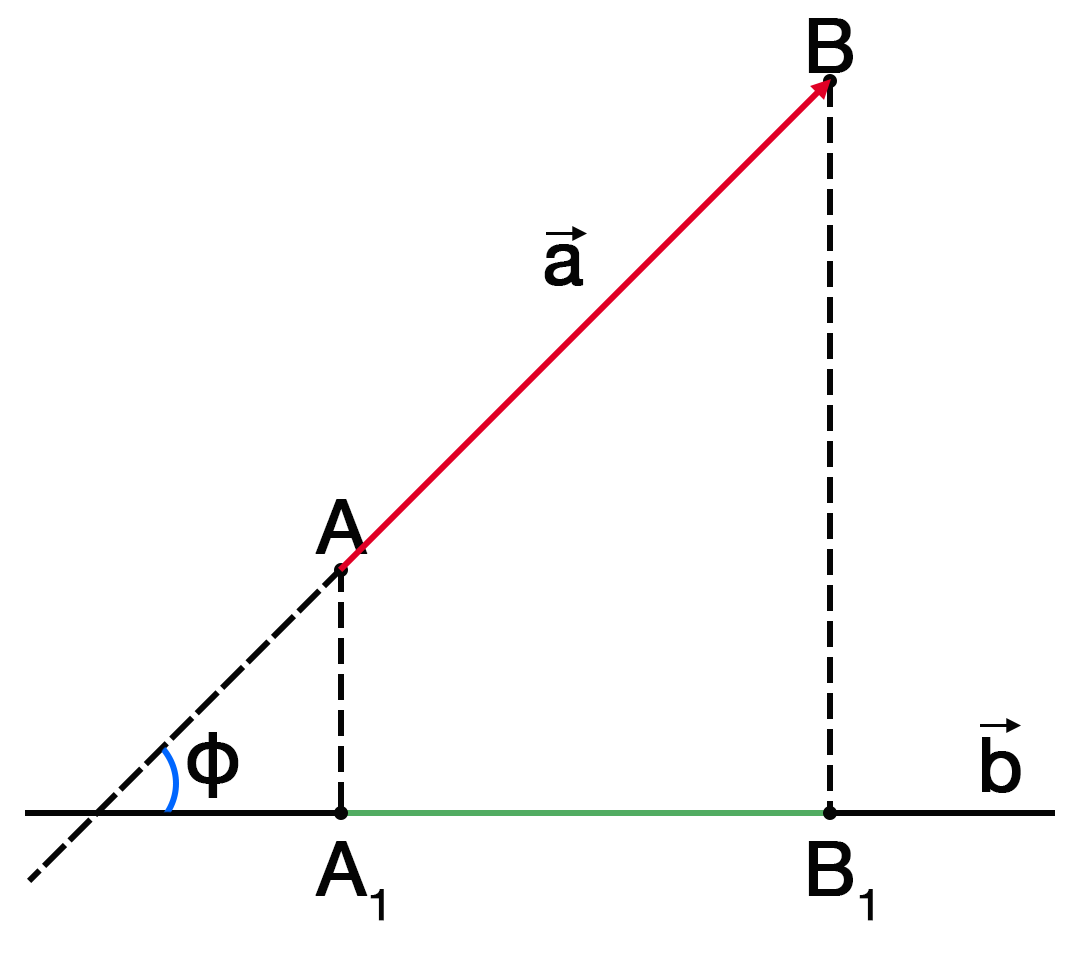
\includegraphics[width=0.5\textwidth]{projection.png}
\end{center}

Проекция вектора \(\vv{AB} = \vv{a}\) обозначается формулой: \(\text{Пр}_{\vv{b}}\vv{AB}\) или \(\text{Пр}_{\vv{b}}\vv{a}\)

Проекция вектора \(\vv{a}\) на ось \(\vv{b}\) выражается формулой:
\begin{gather*}
    \text{Пр}_{\vv{b}}\vv{a} = |\vv{a}| \cdot \cos{\varphi}
\end{gather*}

С другой стороны:
\begin{gather*}
    \cos{\varphi} = \frac{\vv{a} \cdot \vv{b}}{|\vv{a}| \cdot |\vv{b}|}
\end{gather*}

Следовательно:
\begin{gather*}
    \text{Пр}_{\vv{b}}\vv{a} = |\vv{a}| \cdot \cos{\varphi} \iff
    \text{Пр}_{\vv{b}}\vv{a} = \frac{|\vv{a}| \cdot \vv{a} \cdot \vv{b}}{|\vv{a}| \cdot \vv{b}} \iff
    \text{Пр}_{\vv{b}}\vv{a} =
    \frac{\vv{a} \cdot \vv{b}}{|\vv{b}|}
\end{gather*}

\subsection*{Свойства проекций}
\begin{enumerate}
    \item {
          \(    \text{Пр}_{\vv{b}}(\vv{a_1} + \vv{a_2} + \vv{a_3}) =
          \text{Пр}_{\vv{b}}\vv{a_1} +
          \text{Пр}_{\vv{b}}\vv{a_2} +
          \text{Пр}_{\vv{b}}\vv{a_3}
          \)
          }
    \item {
          \(
          \text{Пр}_{\vv{b}}(\lambda \cdot \vv{a}) = \lambda \cdot \text{Пр}_{\vv{b}}\vv{a}
          \)
          }
\end{enumerate}


\section{Векторное произведение и его свойства}%
\label{sec:Векторное произведение и его свойства}

\begin{definition}
    Векторным произведением \(\vv{a}\) на \(\vv{b}\) называется \(\vv{c}\), \textbf{длина} которого численно \textbf{равна площади параллелограмма}, построенного на \(\vv{a}\) и \(\vv{b}\), перпендикулярного к плоскости этих векторов и направленного так, чтоб \textbf{наименьшее вращение} от \(\vv{a}\) к \(\vv{b}\) вокруг вектора \(\vv{c}\) осуществлялось \textbf{против часовой} стрелки, если смотреть с конца \(\vv{c}\):

    \begin{center}
        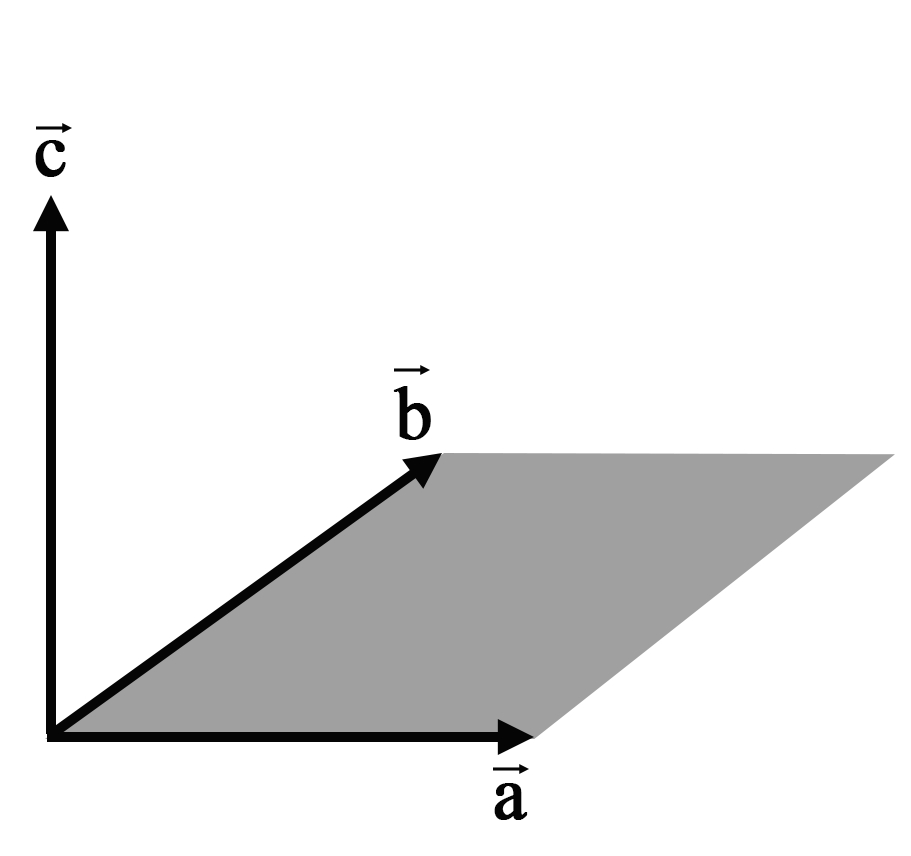
\includegraphics[width=0.4\textwidth]{vector_product.png}
    \end{center}

    Векторное произведение обозначается либо как \(\vv{a} \times \vv{b}\), либо как \([\vv{a}, \vv{b}]\).
\end{definition}

\subsection*{Вычисление векторного произведения}%
\label{sub:Вычисление векторного произведения}
Векторное произведение двух векторов \(\vv{a} = (a_x; a_y; a_z)\) и \(\vv{b} = (b_x; b_y; b_z)\) в декартовой системе координат — это \textbf{вектор}, значение которого можно вычислить по формуле:
\[
    \vv{a} \times \vv{b} =
    \begin{vmatrix}
        i   & j   & k   \\
        a_x & a_y & a_z \\
        b_x & b_y & b_z
    \end{vmatrix}
    = (a_y b_z - a_z b_y)\vv{i} - (a_x b_z - a_z b_x)\vv{j} + (a_x b_y - a_y b_x)\vv{k}
\]
\[
    \vv{a} \times \vv{b} = (a_y b_z - a_z b_y, a_z b_x - a_x b_z, a_x b_y - a_y b_x)
\]

\subsection*{Геометрический смысл векторного произведения}%
\label{sub:Геометрический смысл векторного произведения}
Модуль векторного произведения двух векторов \(\vv{a}\) и \(\vv{b}\) равен площади параллелограмма, построенного на этих векторах:
\[
    S_{\text{парал-ма}} = |\vv{a} \times \vv{b}|
\]
Как следствие, площадь треугольника, построенного на этих же векторах равна половине модуля векторного произведения:
\[
    S_{\Delta} = \frac{1}{2} |\vv{a} \times \vv{b}|
\]

\subsection*{Свойства векторного произведения}%
\label{sub:Свойства векторного произведения}

\begin{enumerate}
    \item {\(\vv{a} \times \vv{b} = - \vv{b} \times \vv{a}\)}

    \item {\((k \vv{a}) \times \vv{b} = \vv{a} \times (k \vv{b}) = k(\vv{a} \times \vv{b})\)}

    \item {\((\vv{a} + \vv{b}) \times \vv{c} = \vv{a} \times \vv{c} + \vv{b} \times \vv{c}\)}

    \item {\(\vv{a} \neq \vv{0}, \vv{b} \neq \vv{0}, \vv{a} \times \vv{b} = 0 \implies \vv{a} || \vv{b}\)}

    \item {\(\vv{a} \neq \vv{0}, \vv{b} \neq \vv{0}, \vv{c} = \vv{a} \times \vv{b} \implies \vv{c} \perp \vv{a}, \vv{c} \perp \vv{b} \)}
\end{enumerate}

\section{Смешанное произведение векторов и его свойства}%
\label{sec:Смешанное произведение векторов и его свойства}

\begin{definition}
    Смешанное произведение векторов — это скалярное произведение вектора \(\vv{a}\) на векторное произведение векторов \(\vv{b}\) и \(\vv{c}\):
    \[
        \vv{a} \cdot (\vv{b} \times \vv{c})
    \]
    Смешанное произведение обозначается либо как \(\vv{a} \cdot (\vv{b} \times \vv{c})\), либо как \((\vv{a}, \vv{b}, \vv{c})\).
\end{definition}

\subsection*{Вычисление смешанного произведения}%
\label{sub:Вычисление смешанного произведения}

Пусть даны векторы \(\vv{a} = (a_x, a_y, a_z)\), \(\vv{b} = (b_x, b_y, b_z)\), \(\vv{c} = (c_x, c_y, c_z)\), тогда их смешанное произведение в декартовой системе координат будет равно:
\[
    \vv{a} \cdot (\vv{b} \times \vv{c}) =
    \begin{vmatrix}
        a_x & a_y & a_z \\
        b_x & b_y & b_z \\
        c_x & c_y & c_z
    \end{vmatrix}
\]

\subsection*{Геометрический смысл смешанного произведения}%
\label{sub:Геометрический смысл смешанного произведения}
Модуль смешанного произведения векторов \(\vv{a}\), \(\vv{b}\), \(\vv{c}\) равен объему параллелепипеда, образованного этими векторами:
\[
    V_{\text{парал-да}} = |\vv{a} \cdot (\vv{b} \times \vv{c})|
\]

Как следствие, объем пирамиды, образованной на этих же векторах равна одной шестой модуля смешанного произведения:
\[
    V_{\text{пирамиды}} = |\vv{a} \cdot (\vv{b} \times \vv{c})|
\]

\subsection*{Алгебраические свойства смешанного произведения}%
\label{sub:Алгебраические свойства смешанного произведения}
\begin{enumerate}
    \item {\(\vv{a} \cdot (\vv{b} \times \vv{c}) = \vv{b} \cdot (\vv{c} \times \vv{a}) = \vv{c} \cdot (\vv{a} \times \vv{b})\)}

    \item {\(\vv{a} \cdot (\vv{b} \times \vv{c}) = - \vv{a} \cdot (\vv{c} \times \vv{b})\)}

    \item {\(\vv{a} \cdot (\vv{b} \times \vv{c}) = (\vv{a} \times \vv{b}) \cdot \vv{c}\)}
\end{enumerate}

\begin{proof}
    \begin{enumerate}
        \item {Длины векторов \(\vv{a}\), \(\vv{b}\), \(\vv{c}\) и ориентация тройки не меняются.}

        \item {Модули слева и справа равны, а ориентация изменилась при перестановке \(\vv{b}\) и \(\vv{c}\) местами.}

        \item {Следует из свойств (1) и (2).}
    \end{enumerate}
\end{proof}


\subsection*{Геометрические свойства смешанного произведения}%
\label{sub:Геометрические свойства смешанного произведения}

\begin{theorem}
    \newpar
    Векторы \(\vv{a}\), \(\vv{b}\), \(\vv{c}\) компланарны тогда и только тогда, когда их смешанное произведение равно нулю.
\end{theorem}

\begin{proof}
    Пусть \((\vv{a}, \vv{b}, \vv{c}) = 0\), тогда может быть два случая:

    \textbf{Случай 1.} \(\vv{b} \times \vv{c} = 0 \implies \vv{b} || \vv{c}\)
    \[
        \text{Тогда} \quad \exists k_1, k_2: \vv{c} = k_1 \vv{a} + k_2 \vv{b} \implies \text{коллинеарность — компланарность.}
    \]

    \textbf{Случай 2.} \(\vv{a} \perp (\vv{b} \times \vv{c})\)

    Доказательство следует напрямую из векторного произведения:
    \[
        \vv{a} \perp (\vv{b} \times \vv{c}) \implies \vv{a} \subset \alpha_{(\vv{b}, \vv{c})} \implies \text{векторы компланарны}
    \]

    Верно и обратное:
    \[
        \vv{a}, \vv{b}, \vv{c} \text{ компланарны }, \vv{a} \perp (\vv{b} \times \vv{c}) \implies
        \vv{a} \cdot (\vv{b} \times \vv{c}) = 0.
    \]
\end{proof}

\subsection*{Алгебраические свойства смешанного произведения}%
\label{sub:Алгебраические свойства смешанного произведения}

\section{Определители 2-го и 3-го порядка. Разложение определителя по элементам строки.}%
\label{sec:Определители 2-го и 3-го порядка}


\section{Свойства определителей}%
\label{sec:Свойства определителей}

1. Определитель транспонированной матрицы равен определителю исходной матрицы: \(\det A^T = \det A\)

2. Умножение всех элементов строки или столбца определителя на некоторое число \(\lambda\) равносильно умножению определителя на это число:
\begin{gather*}
    \begin{vmatrix}
        a_{11}         & a_{12}         & \dots a_{1j}         & \dots & a_{1n}         \\
        a_{21}         & a_{22}         & \dots a_{2j}         & \dots & a_{2n}         \\
        \dots          & \dots          & \dots                & \dots & \dots          \\
        \lambda a_{i1} & \lambda a_{i2} & \dots \lambda a_{ij} & \dots & \lambda a_{in} \\
        \dots          & \dots          & \dots                & \dots & \dots          \\
        a_{m1}         & a_{m2}         & \dots a_{mj}         & \dots & a_{mn}         \\
    \end{vmatrix}
    =
    \lambda \cdot
    \begin{vmatrix}
        a_{11} & a_{12} & \dots a_{1j} & \dots & a_{1n} \\
        a_{21} & a_{22} & \dots a_{2j} & \dots & a_{2n} \\
        \dots  & \dots  & \dots        & \dots & \dots  \\
        a_{i1} & a_{i2} & \dots a_{ij} & \dots & a_{in} \\
        \dots  & \dots  & \dots        & \dots & \dots  \\
        a_{m1} & a_{m2} & \dots a_{mj} & \dots & a_{mn} \\
    \end{vmatrix}
\end{gather*}

3. Если в определителе переставить местами любые две строки или два столбца, то определитель изменяет свой знак на противоположный:
\begin{gather*}
    \begin{vmatrix}
        \dots  & \dots  & \dots  & \dots & \dots  \\
        a_{i1} & a_{i2} & a_{i3} & \dots & a_{in} \\
        \dots  & \dots  & \dots  & \dots & \dots  \\
        a_{k1} & a_{k2} & a_{k3} & \dots & a_{kn} \\
        \dots  & \dots  & \dots  & \dots & \dots  \\
    \end{vmatrix}
    =
    -
    \begin{vmatrix}
        \dots  & \dots  & \dots  & \dots & \dots  \\
        a_{k1} & a_{k2} & a_{k3} & \dots & a_{kn} \\
        \dots  & \dots  & \dots  & \dots & \dots  \\
        a_{i1} & a_{i2} & a_{i3} & \dots & a_{in} \\
        \dots  & \dots  & \dots  & \dots & \dots  \\
    \end{vmatrix}
\end{gather*}

4. Если матрица содержит нулевую строку (столбец), то определитель этой матрицы равен нулю:
\begin{gather*}
    \begin{vmatrix}
        \dots  & \dots  & \dots  & \dots & \dots  \\
        a_{i1} & a_{i2} & a_{i3} & \dots & a_{in} \\
        0      & 0      & 0      & \dots & 0      \\
        a_{j1} & a_{j2} & a_{j3} & \dots & a_{jn} \\
        \dots  & \dots  & \dots  & \dots & \dots  \\
    \end{vmatrix}
    = 0
\end{gather*}

5. Если две строки (столбца) матрицы равны между собой, то определитель этой матрицы равен нулю:
\begin{gather*}
    \begin{vmatrix}
        \dots  & \dots  & \dots  & \dots & \dots  \\
        a_{i1} & a_{i2} & a_{i3} & \dots & a_{in} \\
        \dots  & \dots  & \dots  & \dots & \dots  \\
        a_{i1} & a_{i2} & a_{i3} & \dots & a_{in} \\
        \dots  & \dots  & \dots  & \dots & \dots  \\
    \end{vmatrix}
    = 0
\end{gather*}

6. Если две строки (столбца) матрицы пропорциональны друг другу, то определитель этой матрицы равен нулю:
\begin{gather*}
    \begin{vmatrix}
        \dots   & \dots   & \dots   & \dots & \dots   \\
        a_{i1}  & a_{i2}  & a_{i3}  & \dots & a_{in}  \\
        \dots   & \dots   & \dots   & \dots & \dots   \\
        ca_{i1} & ca_{i2} & ca_{i3} & \dots & ca_{in} \\
        \dots   & \dots   & \dots   & \dots & \dots   \\
    \end{vmatrix}
    = 0
\end{gather*}

7. Определитель матрицы треугольного вида равен произведению элементов, стоящих на главной диагонали:
\begin{gather*}
    \begin{vmatrix}
        a_{11} & a_{12} & a_{13} & \dots & a_{1n} \\
        0      & a_{22} & a_{23} & \dots & a_{2n} \\
        0      & 0      & a_{33} & \dots & a_{3n} \\
        \dots  & \dots  & \dots  & \dots & \dots  \\
        0      & 0      & 0      & \dots & a_{mn} \\
    \end{vmatrix}
    = a_{11} \cdot a_{22} \cdot a_{33} \cdot ... \cdot a_{mn}
\end{gather*}

8. Если все элементы k-ой строки (столбца) определителя представлены в виде сумм \(a_{kj} + b_{kj}\), то определитель можно представить в виде суммы соответствующих определителей:
\begin{gather*}
    \hspace{0.9cm}
    \begin{vmatrix}
        a_{11}          & a_{12}          & a_{13}          & \dots & a_{1n}          \\
        \dots           & \dots           & \dots           & \dots & \dots           \\
        a_{k1} + b_{k1} & a_{k2} + b_{k2} & a_{k3} + b_{k3} & \dots & a_{kn} + b_{kn} \\
        \dots           & \dots           & \dots           & \dots & \dots           \\
        a_{m1}          & a_{m2}          & a_{m3}          & \dots & a_{mn}          \\
    \end{vmatrix}
    =
    \\
    =
    \begin{vmatrix}
        a_{11} & a_{12} & a_{13} & \dots & a_{1n} \\
        \dots  & \dots  & \dots  & \dots & \dots  \\
        a_{k1} & a_{k2} & a_{k3} & \dots & a_{kn} \\
        \dots  & \dots  & \dots  & \dots & \dots  \\
        a_{m1} & a_{m2} & a_{m3} & \dots & a_{mn} \\
    \end{vmatrix}
    +
    \begin{vmatrix}
        a_{11} & a_{12} & a_{13} & \dots & a_{1n} \\
        \dots  & \dots  & \dots  & \dots & \dots  \\
        b_{k1} & b_{k2} & b_{k3} & \dots & b_{kn} \\
        \dots  & \dots  & \dots  & \dots & \dots  \\
        a_{m1} & a_{m2} & a_{m3} & \dots & a_{mn} \\
    \end{vmatrix}
\end{gather*}

9. Определитель не изменится, если к элементам любой его строки (или столбца) прибавить соответствующие элементы другой строки (или соответствующего столбца), умноженные на одно и тоже число:
\begin{gather*}
    \begin{vmatrix}
        \dots  & \dots  & \dots  & \dots & \dots  \\
        a_{i1} & a_{i2} & a_{i3} & \dots & a_{in} \\
        \dots  & \dots  & \dots  & \dots & \dots  \\
        a_{k1} & a_{k2} & a_{k3} & \dots & a_{kn} \\
        \dots  & \dots  & \dots  & \dots & \dots  \\
    \end{vmatrix}
    =
    \begin{vmatrix}
        \dots            & \dots            & \dots            & \dots & \dots            \\
        a_{i1}           & a_{i2}           & a_{i3}           & \dots & a_{in}           \\
        \dots            & \dots            & \dots            & \dots & \dots            \\
        a_{k1} + ca_{i1} & a_{k2} + ca_{i2} & a_{k3} + ca_{i3} & \dots & a_{kn} + ca_{in} \\
        \dots            & \dots            & \dots            & \dots & \dots            \\
    \end{vmatrix}
\end{gather*}

10. Пусть A и B – квадратные матрицы одного и того же порядка. Тогда определитель произведения матриц равен произведению определителей:
\begin{gather*}
    \det (AB) = \det A \cdot \det B
\end{gather*}

\section{Теорема Крамера}%
\label{sec:Теорема Крамера}

\textbf{Метод крамера} (правило Крамера) — способ решения систем линейных алгебраических уравнений с \textbf{числом уравнений равным числу неизвестных} с \underline{ненулевым} главным определителем матрицы коэффициентов системы (причём для таких уравнений решение существует и единственно).

\begin{theorem}[Крамера]
    \newpar
    Для системы линейных уравнения вида:

    \begin{gather*}
        \begin{cases}
            \begin{matrix}
                a_{11}x_1 & +      & a_{12}x_2 & +      & \cdots & +      & a_{1n}x_n & =      & b_1    \\
                a_{21}x_1 & +      & a_{22}x_2 & +      & \cdots & +      & a_{2n}x_n & =      & b_2    \\
                \cdots    & \cdots & \cdots    & \cdots & \cdots & \cdots & \cdots    & \cdots & \cdots \\
                a_{n1}x_1 & +      & a_{n2}x_2 & +      & \cdots & +      & a_{nn}x_n & =      & b_n
            \end{matrix}
        \end{cases}
    \end{gather*}

    Матрица коэффициентов:

    \begin{equation*}
        A = \left(
        \begin{array}{cccc}
            a_{11} & a_{12} & \cdots & a_{1n} \\
            a_{21} & a_{22} & \cdots & a_{2n} \\
            \cdots & \cdots & \cdots & \cdots \\
            a_{n1} & a_{n2} & \cdots & a_{nn}
        \end{array}
        \right)
    \end{equation*}

    Матрица правых частей:

    \begin{equation*}
        B = \left(
        \begin{array}{cccc}
            b_{1}  \\
            b_{2}  \\
            \cdots \\
            b_{n}
        \end{array}
        \right)
    \end{equation*}

    Справедливо утверждение:

    \begin{equation*}
        x_k = \frac{\det C_k}{\det A} \text{ где } k = 1, 2, \dots, n.
    \end{equation*}

    \(C_k\) — матрица, получаемая заменой \(k\)-го столбца матрицы \(A\) столбцом \(B\).
\end{theorem}

\begin{proof}

    Рассмотрим систему уравнений:

    \begin{gather*}
        \begin{cases}
            a_{11}x_1 + a_{12}x_2 = b_1 \\
            a_{21}x_1 + a_{22}x_2 = b_2
        \end{cases}
    \end{gather*}

    Тогда:

    \begin{gather*}
        \begin{cases}
            x_1 = \dfrac{a_{11}b_1 - a_{12}b_1}{a_{11}a_{22} - a_{21}a_{12}} = \dfrac{\Delta{x_1}}{\Delta}
            \vspace{0.5cm} \\
            x_2 = \dfrac{a_{11}b_2 - a_{21}b_1}{a_{11}a_{22} - a_{21}a_{12}} = \dfrac{\Delta{x_2}}{\Delta}
        \end{cases}
    \end{gather*}

    где:

    \begin{equation*}
        \Delta =
        \begin{vmatrix}
            a_{11} & a_{12} \\
            a_{21} & a_{22}
        \end{vmatrix}
        \qquad
        \Delta{x_1} =
        \begin{vmatrix}
            b_{1} & a_{12} \\
            b_{2} & a_{22}
        \end{vmatrix}
        \qquad
        \Delta{x_2} =
        \begin{vmatrix}
            a_{11} & b_{1} \\
            a_{21} & b_{2}
        \end{vmatrix}
    \end{equation*}
\end{proof}

\section{Системы координат. преобразования сдвига и поворота}
\label{sec:coordinate_systems}

\subsection*{Декартова система координат}

Расположение точки \(P\) на плоскости определяется декартовыми координатами с помощью пары чисел \((x, y)\):
\begin{itemize}
    \item {x — расстояоние от точки \(P\) до оси \(y\) с учетом знака}
    \item {y — расстояоние от точки \(P\) до оси \(x\) с учетом знака}
\end{itemize}

\begin{center}
    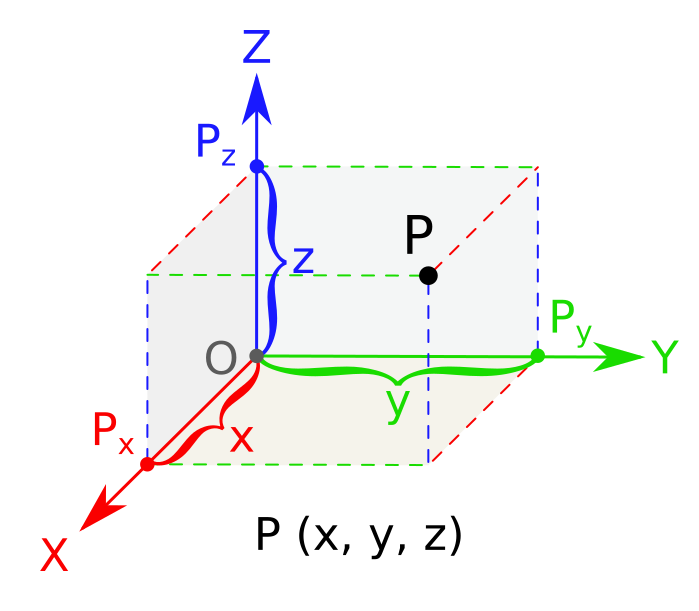
\includegraphics[width=0.6\textwidth]{cartesian_system.png}
\end{center}

В пространстве уже необходимы три координаты \((x, y, z)\) :
\begin{itemize}
    \item {x — расстояоние от точки \(P\) до плоскости \(yz\)}
    \item {y — расстояоние от точки \(P\) до плоскости \(xz\)}
    \item {z — расстояоние от точки \(P\) до плоскости \(xy\)}
\end{itemize}

\subsection*{Полярная система координат}
Полярная система координат задаётся лучом, который называют \textbf{нулевым лучом} или \textbf{полярной осью}.
В нашем случае полярная ось совпадает с осью \(Ox\).
Точка, из которой выходит этот луч, называется \textbf{началом координат} или \textbf{полюсом}.
На схеме таковой точкой является точка \(O\).

Пусть \(M (r, \varphi)\) — произвольная точка в полярной системе координат.
Положение точки \(M\) фиксируется двумя числами: \textbf{радиусом} \(r = \vv{OM}\) и углом \(\varphi\) между полярной осью и вектором \(\vv{OM}\).
Этот угол называется \textbf{полярным углом}.

\begin{center}
    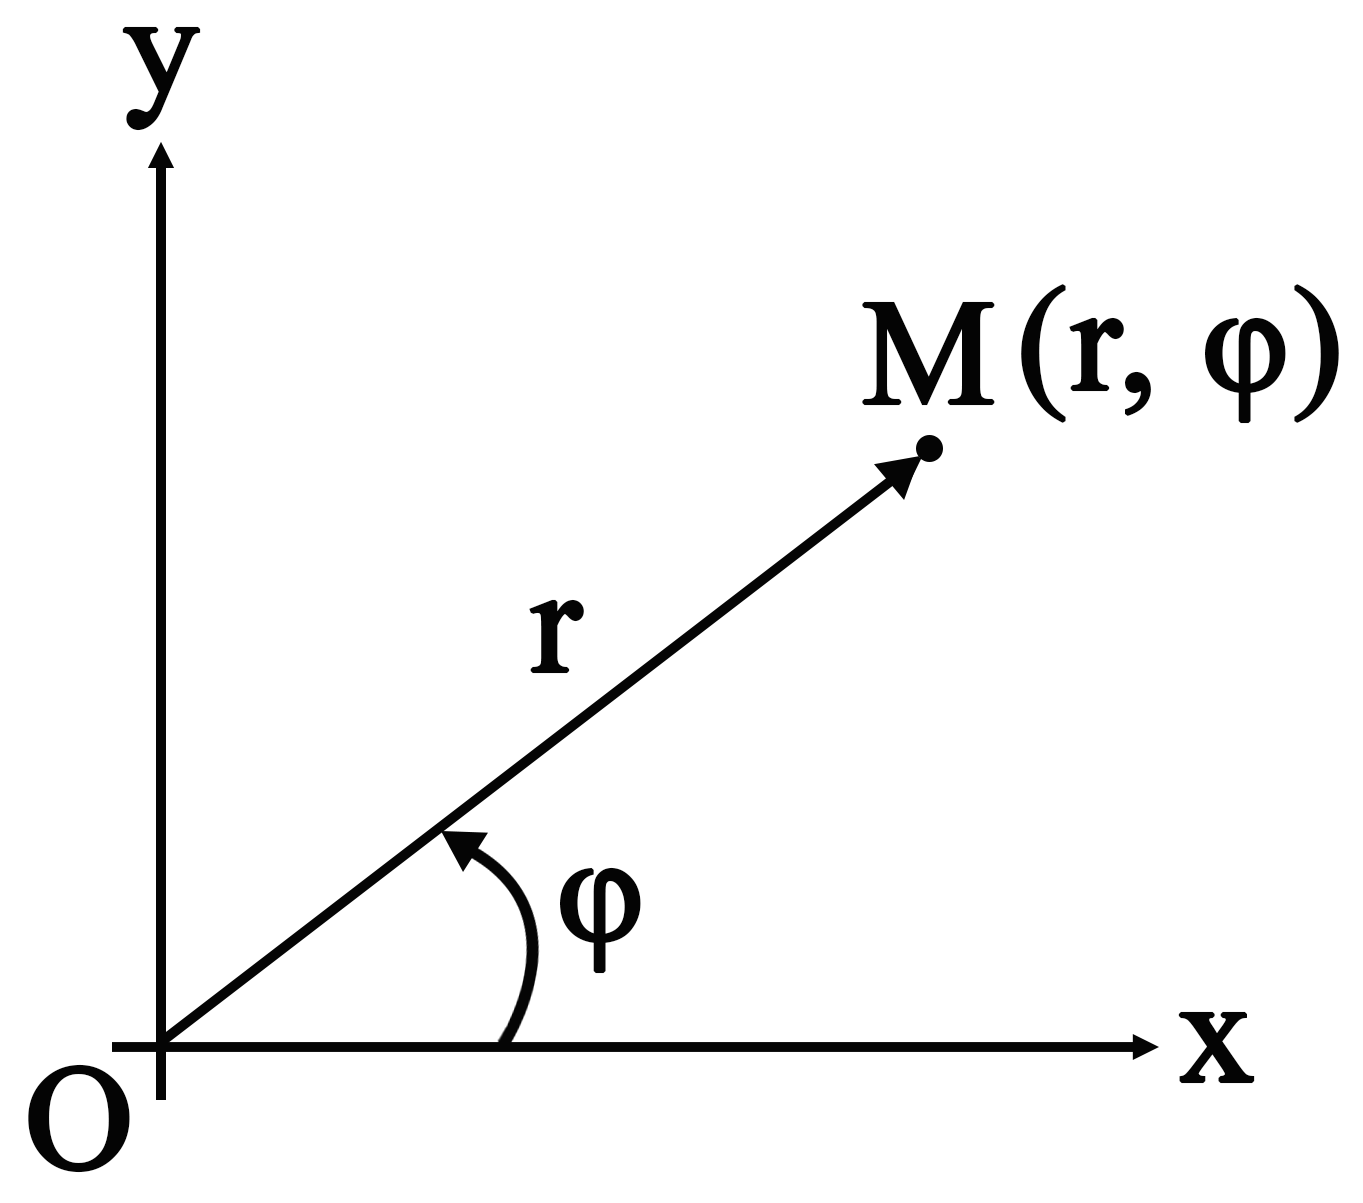
\includegraphics[width=0.5\textwidth]{polar_system.png}
\end{center}

Декартовы координаты точки выражаются формулами:
\begin{gather*}
    x = r \cos{\varphi} \\
    y = r \sin{\varphi}
\end{gather*}

\subsubsection*{Обозначения и ограничения}
\begin{itemize}
    \item {\(r \geq 0\) — радиус (также обозначают за \(r\))}
    \item {\(0 \leq \varphi < 2\pi\) или \(-\pi < \varphi \leq \pi\) — азимут или долгота (также обозначают за \(\theta\))}
    \item {\(h\) — высота (также обозначают за \(z\))}
\end{itemize}

Полярный радиус определен для любой точки плоскости и всегда принимает неотрицательные значения \(r \geq 0\).

Полярный угол \(\varphi\) определен для любой точки плоскости, за исключением полюса \(O\), и принимает значения \(-\pi < \varphi \leq \pi\), то есть координаты \((r, \varphi + 2\pi)\) и  \((r, \varphi + 4\pi)\) соответствуют одной точке.
Полярный угол отсчитывается от полярной оси против часовой стрелки и измеряется в радианах.

\subsubsection*{Достоинства}
Полярная система координат особенно полезна в случаях, когда отношения между точками проще изобразить в виде радиусов и углов; в более распространённой декартовой, или прямоугольной, системе координат, такие отношения можно установить только путём применения тригонометрических уравнений.

\subsubsection*{Недостатки}
\begin{itemize}
    \item Угол \(\varphi\) не определен, если \(r = 0\).
\end{itemize}

\subsection*{Цилиндрическая система координат}
Цилиндрические координаты — трёхмерный аналог полярных координат,
являющуюся расширением полярной системы координат путём добавления третьей координаты (обычно обозначаемой \(h\) или \(z\)), которая задаёт высоту точки над плоскостью.

\begin{center}
    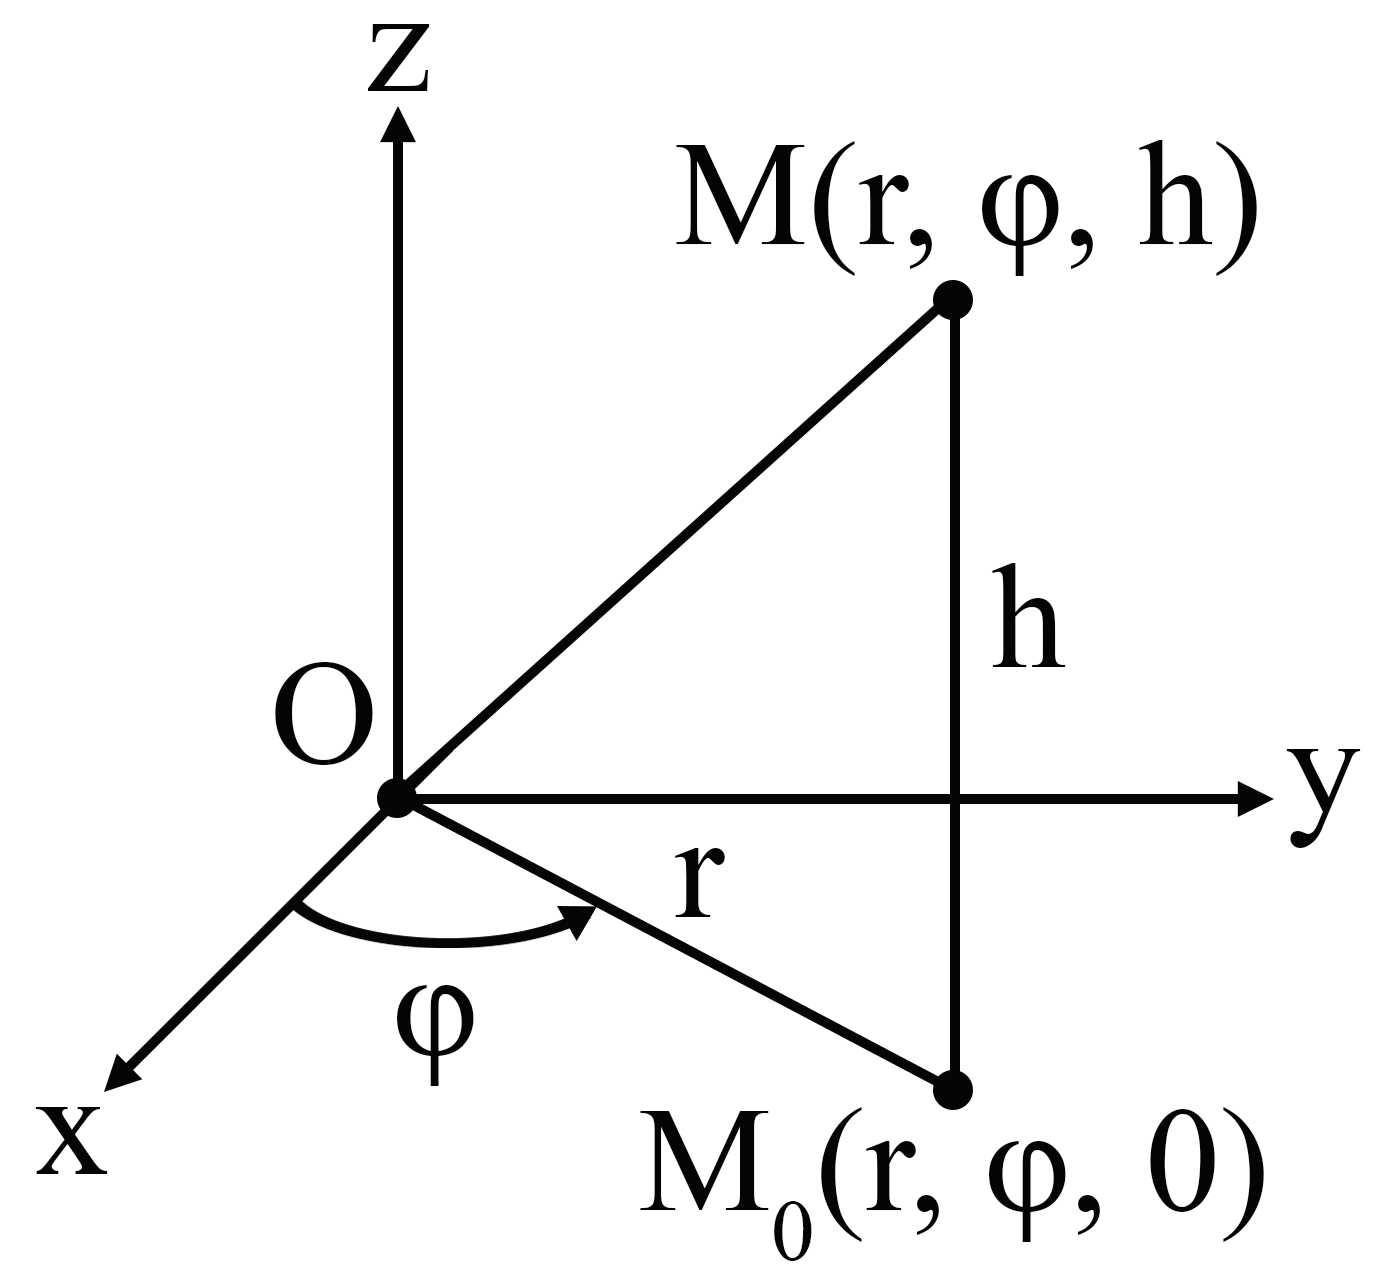
\includegraphics[width=0.5\textwidth]{cylindrical_system.png}
\end{center}

Пусть \(M(r, \varphi, h)\) — произвольная точка циллиндрической системы координат, а \(M_0(r, \varphi, 0)\) — ее проекция на плоскость \(xy\). Тогда:
\begin{itemize}
    \item[]{\(r\) — это расстояние от точки \(M\) до оси \(Oz\)}
    \item[]{\(\varphi\) — угол между осью \(Ox\) и отрезком \(OM_0\)}
    \item[]{\(h\) — расстояние от точки \(M\) до плоскости \(xy\)}
\end{itemize}

\subsubsection*{Обозначения и ограничения}
\begin{itemize}
    \item {\(r \geq 0\) — радиус (также обозначают за \(r\))}
    \item {\(0 \leq \varphi < 2\pi\) или \(-\pi < \varphi \leq \pi\) — азимут или долгота (также обозначают за \(\theta\))}
    \item {\(h\) — высота (также обозначают за \(z\))}
\end{itemize}

\subsubsection*{Достоинства}
Цилиндрические координаты полезны для изучения систем, симметричных относительно некоторой оси. Например, длинный цилиндр с радиусом R в декартовых координатах (с осью z, совпадающей с осью цилиндра) имеет уравнение \(x^2 + y^2 = R^2\), тогда как в цилиндрических координатах оно выглядит гораздо проще, как \(r = R\).

\subsubsection*{Недостатки}
\begin{itemize}
    \item Угол \(\varphi\) не определен, если \(r = 0\).
\end{itemize}

\subsection*{Сферическая система координат}
Сферическая система координат — трёхмерная система координат, в которой каждая точка пространства определяется тремя числами \((r, \varphi, \theta)\).

Пусть \(M(r, \varphi, \theta)\) — произвольная точка сферической системы координат, а \(M_0(r, \varphi, 0)\) — ее проекция на плоскость \(xy\). Тогда:
\begin{itemize}
    \item[]{\(r\) — это расстояние от точки \(M\) до полюса \(O\)}
    \item[]{\(\varphi\) — угол между осью \(Ox\) и отрезком \(OM_0\)}
    \item[]{\(\theta\) — угол между осью \(Oz\) и отрезком \(OM\)}
\end{itemize}

\begin{center}
    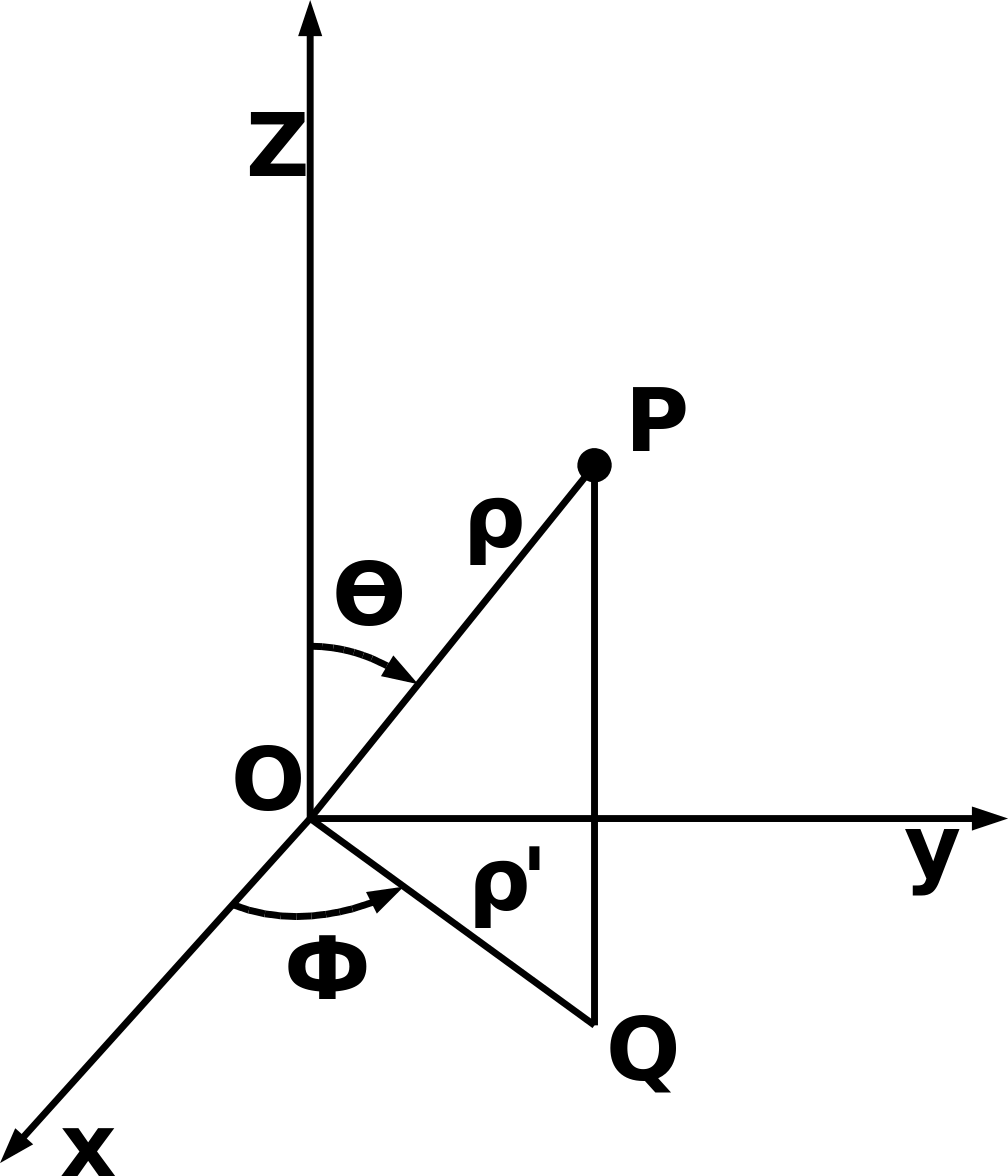
\includegraphics[width=0.5\textwidth]{spherical_system.png}
\end{center}

\subsubsection*{Обозначения и ограничения}
\begin{itemize}
    \item {\(r \geq 0\) — радиус (также обозначают за \(r\))}
    \item {\(0 \leq \varphi < 2\pi\) или \(-\pi < \varphi \leq \pi\) — азимут или долгота (также обозначают за \(\theta\))}
    \item {\(0 \leq \theta \leq \pi\) или \(-\dfrac{\pi}{2} \leq \theta \leq \dfrac{\pi}{2}\) — широта или полярный угол (также обозначают за \(\varphi\))}
\end{itemize}

\subsubsection*{Достоинства}
Сферические координаты полезны при изучении систем, симметричных относительно точки. Так, уравнение сферы с радиусом R в декартовых координатах с началом отсчёта в центре сферы выглядит как \(x^2 + y^2 = R^2\), тогда как в сферических координатах оно становится намного проще: \(r = R\).

\subsubsection*{Недостатки}
\begin{itemize}
    \item Углы \(\varphi\) и \(\theta\) не определены, если \(r = 0\).
    \item Угол \(\varphi\) неопределен для граничных значений \(\theta = 0\) и \(\theta = \pi\) (или для \(\theta = \pm \dfrac{\pi}{2}\), при \(-\dfrac{\pi}{2} \leq \theta \leq \dfrac{\pi}{2}\))
\end{itemize}

\section{Плоскость и ее уравнения}\label{sec:plane}

\textbf{Плоскость} – это геометрическая фигура, состоящая из отдельных точек. Каждой точке в трехмерном пространстве соответствуют координаты, которые задаются тремя числами. Уравнение плоскости устанавливает зависимость между координатами всех точек.

\subsection*{Общее уравнение плоскости}
\begin{gather*}
    Ax + By + Cz + D = 0
\end{gather*}
\subsubsection*{Теорема}
Всякая плоскость в прямоугольной системе координат \(Oxyz\) в трехмерном пространстве может быть задана уравнением вида \(Ax + By + Cz + D = 0\), где \(A, B, C, D\) — некоторые действительные числа, одновременно не равные нулю. Всякое уравнение, имеющее вид \(Ax + By + Cz + D = 0\) определяет плоскость в трехмерном пространстве.

% TODO добавить доказательство

\subsection*{Уравнение плоскости в отрезках}
Если плоскость пересекает оси \(OX\), \(OY\), \(OZ\) в точках с координатами \((a, 0, 0)\), \((0, b, 0)\), \((0, 0, c)\), то она может быть найдена по формуле \textbf{уравнения плоскости в отрезках}:
\begin{gather*}
    \frac{x}{a} + \frac{y}{b} + \frac{z}{c} = 1
\end{gather*}

% TODO добавить доказательство

\subsection*{Уравнение плоскости, проходящей через точку, перпендикулярно вектору нормали}
Пусть у нас есть точка \(M(x_0, y_0, z_0)\), принадлежащая плоскости, и вектор нормали плоскости \(\vv{n} = (A, B, C)\). Тогда плоскость задается уравнением:
\begin{gather*}
    A(x - x_0) + B(y - y_0) + C(z - z_0) = 0
\end{gather*}

% TODO добавить доказательство

\subsection*{Уравнение плоскости, проходящей через три заданные точки, не лежащие на одной прямой}
Пусть у нас есть три точки \(A(x_1, y_1, z_1)\), \(B(x_2, y_2, z_2)\), \(C(x_3, y_3, z_3)\), лежащих на плоскости и не лежащих на одной прямой. Тогда уравнение плоскости можно найти по формуле:
\begin{gather*}
    \begin{vmatrix}
        x - x_1   & y - y_1   & z - z_1   \\
        x_2 - x_1 & y_2 - y_1 & z_2 - z_1 \\
        x_3 - x_1 & y_3 - y_1 & z_3 - z_1
    \end{vmatrix}
\end{gather*}

% TODO добавить доказательство

\section{Прямая в пространстве и ее уравнения}\label{sec:line_in_space}
Уравнение прямой на плоскости в прямоугольной системе координат \(Oxy\) – это линейное уравнение с переменными \(x\) и \(y\), которому отвечают координаты всех точек прямой и не удовлетворяют координаты никаких прочих точек.

\subsection*{Уравнение прямой в пространстве как уравнение двух пересекающихся плоскостей}
Когда две плоскости в пространстве имеют общую точку, существует их общая прямая, на которой находятся все общие точки этих плоскостей.

Пусть у нас есть две плоскости \(\alpha\) и \(\beta\), которые описываются следующими уравнениями плоскости:
\begin{gather*}
    \alpha: A_1x + B_1y + C_1z + D_1 = 0 \\
    \beta: A_2x + B_2y + C_2z + D_2 = 0
\end{gather*}

Прямую их пересечения обозначим за \(l\). Поскольку любая точка прямой удовлетворяет сразу двум уравнениям плоскостей, координаты любой точки прямой будут частным решением системы:
\begin{gather*}
    \begin{cases}
        A_1x + B_1y + C_1z + D_1 = 0 \\
        A_2x + B_2y + C_2z + D_2 = 0
    \end{cases}
\end{gather*}

\subsection*{Канонические уравнения прямой в пространстве}
Пусть у нас есть некоторая прямая \(l\), точка \(M_0(x_0, y_0, z_0)\), лежащая на прямой \(l\) и направляющий вектор \(\vv{r} = (m, n, p)\). Пусть \(M(x, y, z)\) — произвольная точка \(l\), тогда вектор \(\vv{M_0M} = (x - x_0, y - y_0, z - z_0)\) и вектор \(r\) коллинеарны. Из условия коллинеарности следует, что:
\begin{gather*}
    \frac{x - x_0}{n} = \frac{y - y_0}{m} = \frac{z - z_0}{p}
\end{gather*}

что является каноническим уравнением прямой в пространстве.

\subsection*{Параметрические уравнения прямой в пространстве}
Воспользуется каноническим уравнением прямой, прировняв каждую из дробей к некоторому параметру \(t\):
\begin{gather*}
    \frac{x - x_0}{n} = \frac{y - y_0}{m} = \frac{z - z_0}{p} = t
\end{gather*}
Тогда получим параметрическое уравнение прямой:
\begin{gather*}
    \begin{cases}
        x = x_0 + nt \\
        y = y_0 + mt \\
        z = z_0 + pt
    \end{cases}
\end{gather*}

\subsection*{Уравнение прямой через две заданные точки}
Пусть даны две точки \(M_1(x_1, y_1, z_1)\) и \(M_2(x_2, y_2, z_2)\), которые лежат на некоторой прямой \(l\). Тогда вектор  \(\vv{M_1M_2} = (x_2 - x_1, y_2 - y_1, z_2 - z_1)\) явлется направляющим вектором этой прямой.

Пусть у нас есть произвольная точка \(M(x, y, z)\), лежащая на прямой \(l\). Тогда вектор \(\vv{M_1M} = (x - x_1, y - y_1, z - z_1)\) будет коллинеарен вектору \(\vv{M_1M_2}\). Из условия коллинеарности следует, что:
\begin{gather*}
    \frac{x - x_1}{x_2 - x_1} = \frac{y - y_1}{y_2 - y_1} = \frac{z - z_1}{z_2 - z_1}
\end{gather*}

что является уравнением прямой в пространстве, которая проходит через две заданные точки.

\section{Прямая на плоскости: уравнение через две точки, каноническое, параметрическое, общее, в отрезках на осях}\label{sec:line_on_plane}

\subsection*{Каноническое уравнение прямой}

Дана прямая \(L\), проходящая через точку \(M_0(x_0;y_0)\), и направляющий вектор \(\vv{a}(m, n)\) этой прямой.
Пусть \(M(x, y)\) — произвольная точка на искомой прямой \(L\), тогда \(M \in L \iff \vv{M_0M} || \vv{a}\).

\begin{center}
    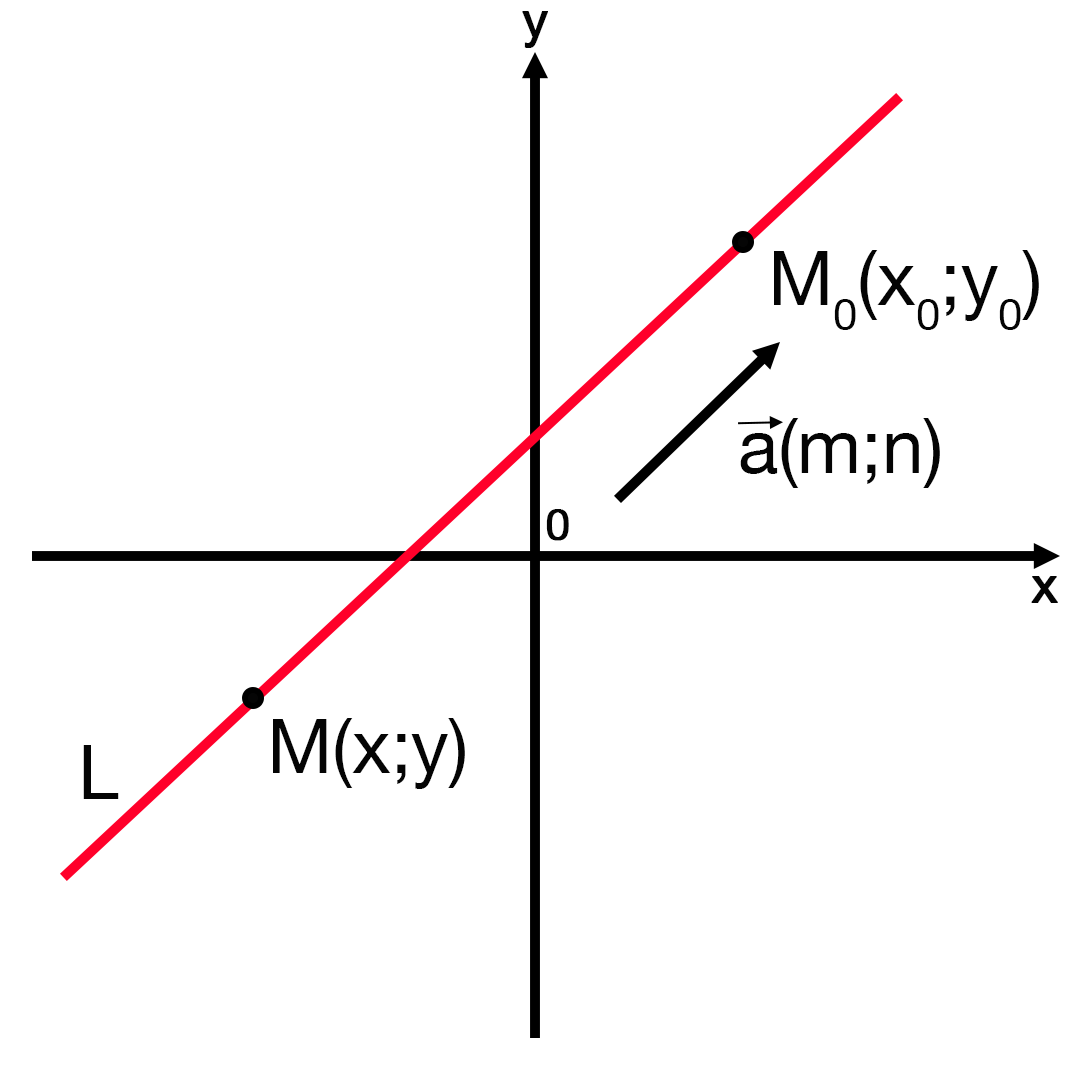
\includegraphics[width=0.5\textwidth]{kanon_line.png}
\end{center}

Условием коллинеарности векторов \(\vv{M_0M}\) и \(\vv{a}\) будет:
\(\dfrac{x - x_0}{m} = \dfrac{y - y_0}{n}\), что и является каноническим уравнением прямой.

\subsection*{Уравнение прямой через 2 заданные точки}

Даны две точки \(M_0(x_0;y_0)\) и \(M_1(x_1;y_1)\), лежащие на прямой \(L\).
Из этого следует, что \(\vv{M_0M_1} = (x_1 - x_0; y_1 - y_0)\) — направляющий вектор прямой \(L\).

Тогда искомое уравнение будет иметь вид: \(\dfrac{x - x_0}{x_1 - x_0} = \dfrac{y - y_0}{y_1 - y_0}\).

\subsection*{Параметрическое уравнение прямой}

Уравнение \(\vv{M_0M} = \lambda \cdot \vv{a}\) называют векторно-параметрическим уравнением прямой, где \lambda — некоторое действительное число.

В векторной форме оно имеет вид:
\begin{gather*}
    \vv{M_0M} = \lambda \cdot \vv{a} \iff
    \begin{cases}
        x - x_0 = \lambda \cdot m \\
        y - y_0 = \lambda \cdot n
    \end{cases}
    \iff
    \begin{cases}
        x = x_0 + \lambda \cdot m \\
        y = y_0 + \lambda \cdot n
    \end{cases}
\end{gather*}

\subsection*{Общее уравнение прямой}

Уравнение, имеющее вид \(Ax + By + C = 0\) — это общее уравнение прямой на плоскости в прямоугольной системе координат \(Oxy\).

\begin{theorem}
    \newpar
    Любое уравнение первой степени, имеющее вид \(Ax + By + C = 0\), где \(A, B, C\) – некоторые действительные числа (\(A\) и \(B\) не равны одновременно нулю) определяет прямую линию в прямоугольной системе координат на плоскости.
    В свою очередь, любая прямая в прямоугольной системе координат на плоскости определяется уравнением, имеющим вид \(Ax + By + C = 0\) при некотором наборе значений \(A, B, C\).
\end{theorem}

\begin{proof}

    Теорема состоит из 2-х пунктов.
    Докажем каждый из них: \\

    \textbf{Пункт 1}. Уравнение \(Ax + By + C = 0\) определяет на плоскости прямую. \\

    Пусть существует некоторая точка \(M_0(x_0, y_0)\), координаты которой отвечают уравнению \(Ax + By + C = 0\), таким образом: \(Ax_0 + By_0 + C = 0\).
    Вычтем из левой и правой частей уравнений \(Ax + By + C = 0\) левую и правую части уравнения \(Ax_0 + By_0 + C = 0\), получим новое уравнение, имеющее вид \(A(x - x_0) + B(y - y_0) + C = 0\).
    Оно эквивалентно \(Ax + By + C = 0\).

    Полученное уравнение \(A(x - x_0) + B(y - y_0) + C = 0\) является необходимым и достаточным условием перпендикулярности векторов \(\vv{n} = (A, B)\) и \(\vv{M_0M} = (x - x_0, y - y_0)\).
    Таким образом множество точек \(M(x, y)\) задает в прямоугольной системе координат прямую линию, перпендикулярную направлению вектора \(\vv{n} = (A, B)\).

    Предположим, что это не так. Тогда вектор \(\vv{n} = (A, B)\) не перпендикулярен вектору \(\vv{M_0M} = (x - x_0, y - y_0)\), а равенство \(A(x - x_0) + B(y - y_0) = 0\) не является верным.

    \begin{center}
        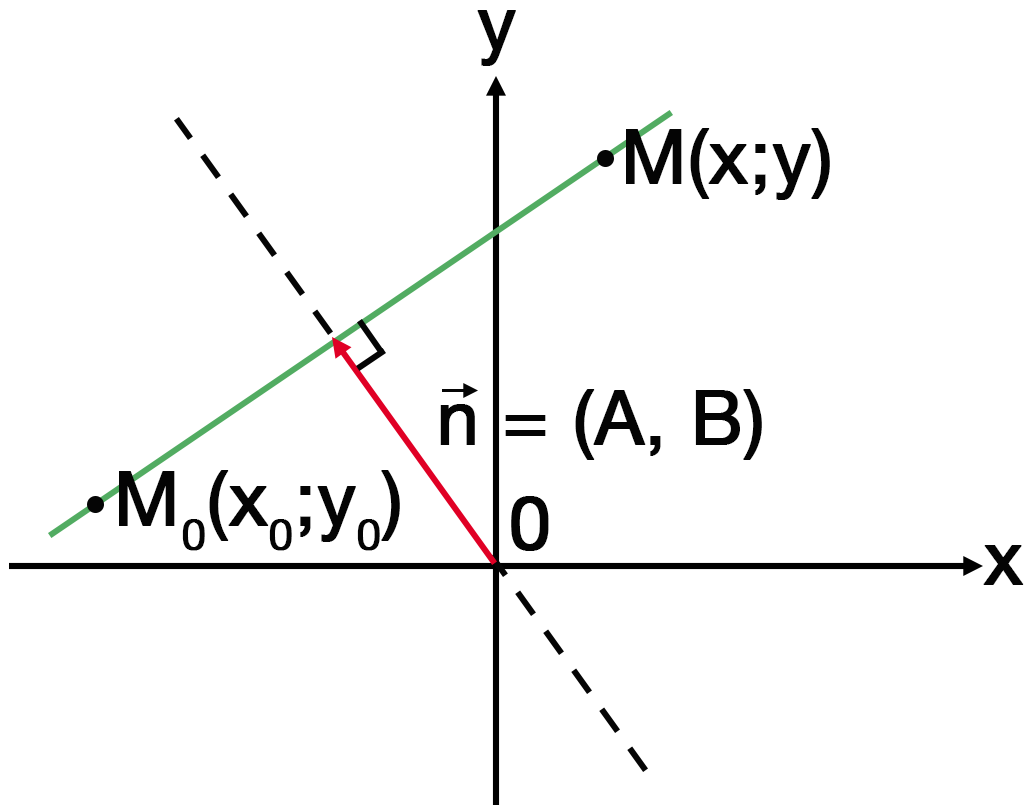
\includegraphics[width=0.5\textwidth]{general_line.png}
    \end{center}

    Следовательно, уравнение \(A(x - x_0) + B(y - y_0) = 0\) определяет некоторую прямую в прямоугольной системе координат на плоскости, а значит и эквивалентное ему уравнение \(Ax + By + C = 0\) определяет ту же прямую. \\

    \textbf{Пункт 2}. Любую прямую в прямоугольной системе координат на плоскости можно задать уравнением первой степени \(Ax + By + C = 0\). \\

    Зададим в прямоугольной системе координат на плоскости прямую \(a \); точку \(M_0(x_0, y_0)\), через которую проходит эта прямая, а также нормальный вектор этой прямой \(\vv{n} = (A, B)\).
    Пусть точка \(M(x, y)\) — произвольная точка на прямой, тогда векторы \(\vv{n} = (A, B)\) и \(\vv{M_0M} = (x - x_0, y - y_0)\) являются перпендикулярными друг другу и их скалярное произведение равно нулю:
    \begin{gather*}
        (\vv{n}, \vv{M_0M}) = A(x - x_0) + B(y - y_0) = 0
    \end{gather*}

    Пусть \(C = -Ax_0 - By_0\), тогда получим уравнение:
    \begin{gather*}
        Ax + By + C = 0
    \end{gather*}
\end{proof}

\subsection*{Уравнение прямой в отрезках на осях}

Рассмотрим общее уравнение прямой \(Ax + By + C = 0\) при условии \(A \neq 0, B \neq 0, C \neq 0\) (то есть прямая не параллельна ни одной из осей координат и не проходит через начало отсчёта).
Теперь преобразуем уравнение:

\begin{gather*}
    Ax + By + C = 0  \iff Ax + By = -C \iff \frac{x}{\frac{-C}{A}} + \frac{y}{\frac{-C}{B}} = 1
\end{gather*}

\begin{center}
    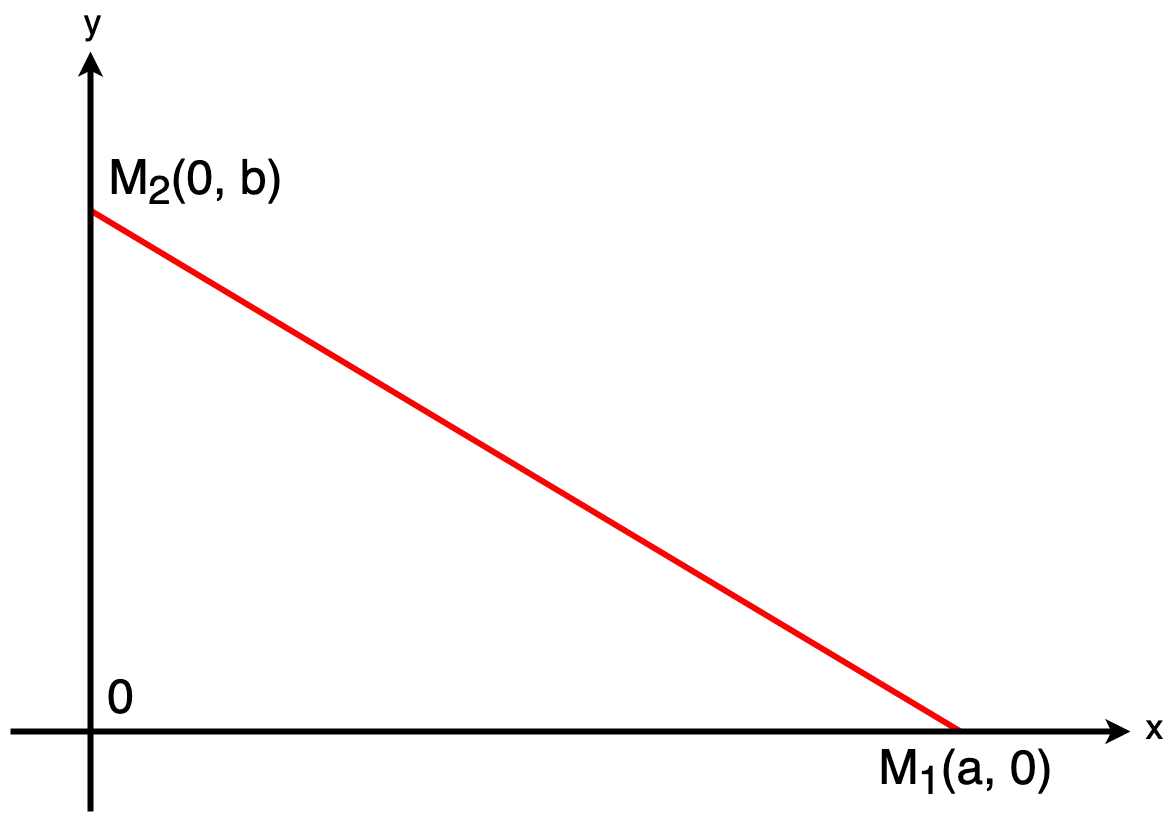
\includegraphics[width=0.7\textwidth]{axis_line.png}
\end{center}

Введем обозначение: \(\frac{-C}{A} = a\), \(\frac{-C}{B} = b\).
Отсюда получим уравнение:
\begin{gather*}
    \frac{x}{a} + \frac{y}{b} = 1
\end{gather*}

Это — уравнение прямой в отрезках на осях, так как числа m и n соответствуют длинам отрезков (с соответствующими знаками), которые прямая отсекает на осях координат (считая от начала отсчёта).

\section{Условия параллельности и перпендикулярности плоскостей и прямых в пространстве}
\label{sec:parallel_perpendicular_planes}

\subsection*{Параллельность и перпендикулярность плоскостей}
Условия параллельности и перпендикулярности двух плоскостей равносильны условиям параллельности и перпендикулярности \textbf{их нормальных векторов}.

Пусть есть две плоскости:
\begin{gather*}
    \alpha: A_1x + B_1y + C_1z + D_1 = 0 \\
    \beta: A_2x + B_2y + C_2z + D_2 = 0
\end{gather*}

Тогда они:
\begin{itemize}
    \item[—]{\textbf{Перпендикулярны}, если \(A_1A_2 + B_1B_2 + C_1C_2 = 0\)}
    \item[—]{\textbf{Параллельны}, когда \(\dfrac{A_1}{A_2} = \dfrac{B_1}{B_2} = \dfrac{C_1}{C_2}\)}
\end{itemize}

\subsection*{Параллельность и перпендикулярность прямых в пространстве}
В пространстве для прямых действуют те же условия, что и на плоскости, добавляется лишь новая координата.

\plink{sec:parallel_perpendicular_lines}{Перейти к параллельности и перпендикулярности прямых в пространстве}

\subsection*{Параллельность и перпендикулярность прямой и плоскости}
Пусть есть прямая:
\begin{gather*}
    l: \frac{x - x_0}{m} = \frac{y - y_0}{n} = \frac{z - z_0}{p}
\end{gather*}

Ее направляющим вектором является вектор \(\vv{s} = (m, n, p)\).

И плоскость:
\begin{gather*}
    \alpha: Ax + By + Cz + D = 0
\end{gather*}

Ее нормальным вектором является вектор \(\vv{n} = (A, B, C)\)

Тогда прямая \textbf{параллельна} плоскости, когда:
\begin{gather*}
    \vv{n} \perp \vv{s} \iff \vv{n} \cdot \vv{s} = 0 \iff Am + Bm + Cp = 0
\end{gather*}

И прямая \textbf{перпендикулярна} плоскости, если:
\begin{gather*}
    \frac{A}{m} = \frac{B}{n} = \frac{C}{p}
\end{gather*}

\section{Условия параллельности и перпендикулярности прямых на плоскости}
\label{sec:parallel_perpendicular_lines}

Условия параллельности и перпендикулярности двух прямых равносильны условиям параллельности и перпендикулярности \textbf{их направляющих векторов}.

\subsection*{Прямые, заданые в общем виде}
Пусть даны прямые, заданные общими уравнениями:
\begin{gather*}
    l_1: A_1x + B_1y + C_1 = 0 \\
    l_2: A_2x + B_2y + C_2 = 0
\end{gather*}

Тогда они:
\begin{itemize}
    \item[—]{\textbf{Перпендикулярны}, если \(A_1A_2 + B_1B_2 = 0\) (условие коллинеарности векторов).}
    \item[—]{\textbf{Параллельны}, когда \(\dfrac{A_1}{A_2} = \dfrac{B_1}{B_2} \neq \dfrac{C_1}{C_2}\) (условие параллельности векторов).}
    \item[—]{\textbf{Совпадают}, если \(\dfrac{A_1}{A_2} = \dfrac{B_1}{B_2} = \dfrac{C_1}{C_2}\).}
\end{itemize}

\subsection*{Прямые с угловым коэффициентом}
Пусть даны прямые:
\begin{gather*}
    l_1: y = k_1x + b_1 \\
    l_2: y = k_2x + b_2
\end{gather*}

Тогда они:
\begin{itemize}
    \item[—]{\textbf{Перпендикулярны}, если \(k_1 = -\dfrac{1}{k_2}\) при \(b_1 \neq b_2\)}
    \item[—]{\textbf{Параллельны}, когда \(k_1 = k_2\)}
\end{itemize}

\subsection*{Прямые, заданные каноническими уравнениями}
Пусть даны прямые, через каноническими уравнениями:
\begin{gather*}
    l_1: \frac{x - x_1}{m_1} = \frac{y - y_1}{n_1} \\
    l_2: \frac{x - x_2}{m_2} = \frac{y - y_2}{n_2}
\end{gather*}

Тогда они:
\begin{itemize}
    \item[—]{\textbf{Перпендикулярны}, когда \(m_1m_2 + n_1n_2 = 0\)}
    \item[—]{\textbf{Параллельны}, если \(\dfrac{m_1}{m_2} = \dfrac{n_1}{n_2}\)}
\end{itemize}

% Рассмотрим прямую с, которая пересекает две прямые а и b и образует с ними восемь углов.
% Такую прямую с называют — секущая.
% Пары углов, которые образует секущая, также имеют названия.
% Итак, на данном рисунке изображены эти все прямые и восемь углов.

% % TODO добавить картинку накр. лежащих и тд

% \begin{enumerate}
%     \item {Если накрест лежащие углы равны (4 и 5, 3 и 6)}
%     \item {Если соответственные углы равны (4 и 6, 3 и 5)}
%     \item {Сумма внутренних односторонних углоав равна 180\textdegree}
% \end{enumerate}

\section{Парабола. Определение, вывод уравнения, характеристики}\label{sec:parabola}

\subsection*{Определение}
Парабола — геометрическое место точек на плоскости, равноудалённых от данной прямой \(d\) и данной точки \(F\).
Точка \(F\) не лежит ни на кривой, ни на прямой \(d\).

Точка \(F\) называется \textbf{фокусом}, а прямая \(d\) — \textbf{директрисой параболы}.
Расстояние от фокуса до директрисы называется \textbf{фокальным параметром} параболы и обозначается через \(p\).

\textbf{Эксцентриситет} параболы — это отношение расстояний от произвольной точки на кривой до фокуса и от этой же точки до директрисы.
Эксцентриситет параболы по определению равен 1.

Каноническое уравнение параболы: \(y^2 = 2px\)

\subsection*{Вывод канонического уравнения}

Пусть фокус \(F\) принадлежит оси \(OX\).
Проведем директрису перпендикулярно оси \(OX\) на расстоянии \(p\) от фокуса \(F\), тогда пусть т. \(O\) будет серединой этого расстояния.
Возьмем т. \(M(x; y)\), которая принадлежит параболе.
Расстояние от т. \(M(x; y)\) до фокуса обозначим за \(r\), до директрисы за \(d\).

\begin{center}
    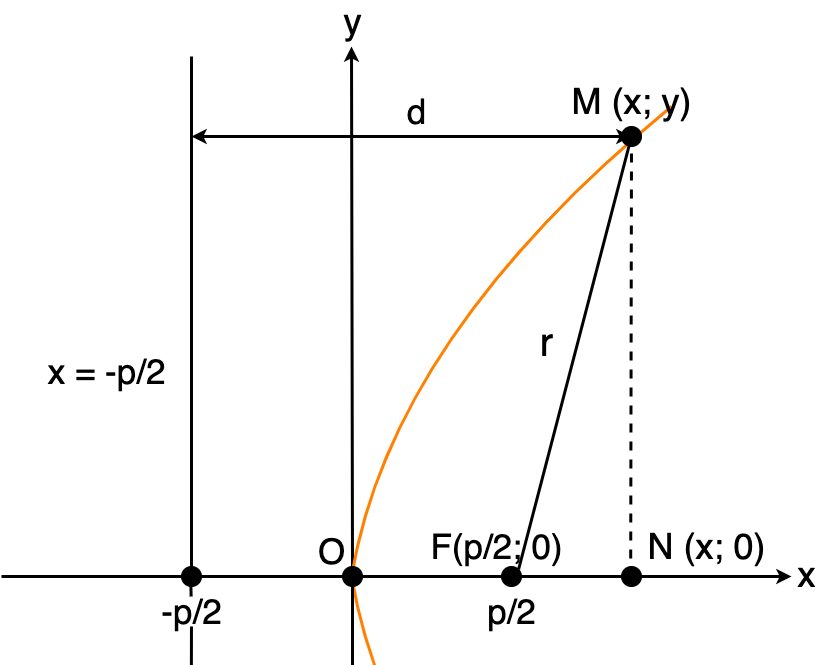
\includegraphics[width=0.8\textwidth]{parabola.png}
\end{center}

Расстояние от т. \(M(x;y)\) до директрисы равно \(d = \Big| x + \dfrac{p}{2} \Big| \).

По определению параболы \(r = d\).

По теореме Пифагора из прямоугольного \(\Delta FMN\): \(r=\sqrt{\Big(x - \dfrac{p}{2}\Big)^2 + y^2}\)

Следовательно:

\begin{gather*}
    \sqrt{\Big(x - \frac{p}{2}\Big)^2 + y^2} = x + \frac{p}{2} \\
    x^2 - px + \frac{p^2}{4} + y^2 = x^2 + px + \frac{p^2}{4} \\
    y^2 = 2px
\end{gather*}

\subsection*{Уравнение в полярной системе координат}

Выберем фокус \(F\) параболы, а в качестве полярной оси — луч с началом в точке \(F\), перпендикулярный директрисе и не пересекающий её.
Тогда для произвольной точки \(M(r, \varphi)\), принадлежащей параболе, по определению \(d = r\).

\begin{center}
    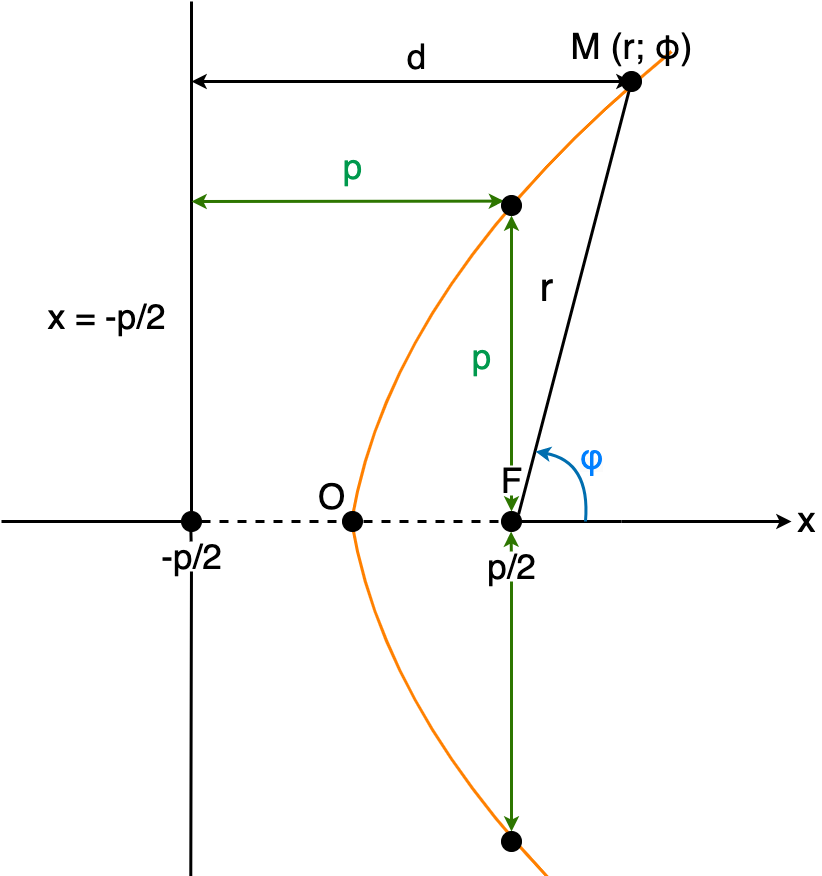
\includegraphics[width=0.7\textwidth]{parabola2.png}
\end{center}

Поскольку \(d = p + r\cos{\varphi}\), получим уравнение параболы в координатной форме:
\begin{gather*}
    d = p + r \cdot \cos{\varphi}  \iff r = \dfrac{p}{1 - \cos{\varphi}}
\end{gather*}

что является уравнением параболы в полярной системе координат \(Fr\varphi\).

\subsection*{Свойства параболы}

\begin{itemize}
    \item[—]{Имеет ось симметрии называемой осью параболы. Ось проходит через фокус и вершину перпендикулярно директрисе;}
    \item[—]{Если фокус параболы отразить относительно касательной, то его образ будет лежать на директрисе;}
    \item[—]{Все параболы подобны. Расстояние между фокусом и директрисой определяет масштаб;}
\end{itemize}

\chapter{Математический анализ}

\section{Вещественная ось. Бесконечность. Окрестность точки}%
\label{sec:Вещественная ось. Бесконечность. Окрестность точки}

\subsection*{Вещественная ось}%
\label{sub:Вещественная ось}
% TODO написать что-нибудь
А что писать сюда???

\subsection*{Бесконечность}%
\label{sub:Бесконечность}
% TODO написать что-нибудь
И сюда что писать?

\subsection*{Окрестность точки}%
\label{sub:Окрестность точки}

\textbf{Окресностью действительной точки} \(x_0\) называется любой открытый интервал, содержащий эту точку:
\[
    U(x_0) = \{x: -\varepsilon_1 < x - x_0 < \varepsilon_2; \varepsilon_1 > 0, \varepsilon_2 > 0\}
\]

\textbf{Эпсилон окрестностью точки} \(x_0\) называется множество точек, расстояние от которых до точки \(x_0\) меньше \(\varepsilon\):
\[
    U(x_0, \varepsilon) = \{x: |x - x_0| < \varepsilon\}
\]

\textbf{Проколотой окрестностью точки} \(x_0\) называется окрестность этой точки, из которой исключили саму эту точку \(x_0\):
\[
    \overset{\circ}{U}(x_0) = U(x_0) \; \backslash \; \{x_0\}
\]

\section{Определения предела функции. Односторонние пределы}%
\label{sec:Определения предела функции. Односторонние пределы}

\subsection*{Предел функции по Коши}%
\label{sub:Предел функции по Коши}

Значение \(A\) называется \textbf{пределом} (\textbf{предельным значением}) функции \(f(x)\) в точке \(x_0\), если для любого положительного числа \(\varepsilon\) можно подобрать соответствующее ему положительное число \(\delta = \delta (\varepsilon)\) такое, что для всех аргументов \(x\), удовлетворяющих условию \(0 < |x - x_0| < \delta\), выполняется неравенство: \(0 \leq |f(x) - A| < \varepsilon\), то есть \(|f(x) -A| < \varepsilon\).

\begin{gather*}
    \lim_{x \to x_0}{f(x)} = A \iff \Big[ \forall \varepsilon > 0: \exists \delta = \delta (\varepsilon) > 0: (0 < |x - x_0| < \delta) \to (|f(x) - A| < \varepsilon) \Big]
\end{gather*}

\subsection*{Окрестностное определение предела по Коши}
Значение \(A\) называется \textbf{пределом} (\textbf{предельным значением}) функции \(f(x)\) в точке \(x_0\), если для любой окрестности \(O(A)\) точки \(A\) существует проколотая окрестность \(\overset{\circ}{O}\) точки \(x_0\) такая, что образ этой окрестности \(f(\overset{\circ}{O}(x_0))\) лежит в \(O(A)\).

\begin{gather*}
    \lim_{x \to x_0}{f(x)} = A \iff \Big[ \forall O(A): \exists \overset{\circ}{O}(x_0): f(\overset{\circ}{O}(x_0) \subseteq O(A)) \Big]
\end{gather*}

\section{Бесконечно малые и бесконечно большие функции}%
\label{sec:Бесконечно малые функции и их свойства}

\subsection*{Бесконечно малые функции и их свойства}%
\label{sub:Бесконечно малые функции и их свойства}

\begin{definition}
    Функция \(\alpha(x)\) называется \textbf{бесконечно малой} при \(x \to x_0\), если \(\displaystyle \exists \lim_{x \to x_0}{\alpha(x)}\) и \(\displaystyle \lim_{x \to x_0}{\alpha(x)} = 0\).
\end{definition}

\subsection*{Свойства бесконечно малых функций}

\begin{property}
    \newpar
    Пусть есть бесконечно малая функция \(\alpha(x)\) при \(x \to x_0\). Также есть функция \(g(x)\), ограниченная в некоторой проколотой окрестности \(\overset{\circ}{U}_g(x_0)\). Тогда их произведение есть бесконечно малая функция:
    \[
        \lim_{x \to x_0}{(\alpha(x) \cdot g(x))} = 0
    \]
\end{property}

\begin{proof}
    Так как \(g(x)\) ограничена в \(\overset{\circ}{U}_g(x_0)\), то \(\exists M: \forall x \in \overset{\circ}{U}_g(x_0) \implies |g(x)| \leq M\).

    Если \(\displaystyle \exists \lim_{x \to x_0}{\alpha(x)}\), то \(\exists \overset{\circ}{U}_\alpha (x_0)\), на которой определена функция \(\alpha(x)\).

    Тогда \(\forall \varepsilon > 0: x \in \overset{\circ}{U}_\alpha(x_0) \implies |\alpha(x)| < \dfrac{\varepsilon}{M}\).

    Пусть \(\overset{\circ}{U}(x_0) = \min(\overset{\circ}{U}_\alpha(x_0), \overset{\circ}{U}_g(x_0))\).

    Тогда
    \(
    \forall \varepsilon > 0: x \in \overset{\circ}{U}(x_0) \implies |\alpha(x) \cdot g(x)| < \dfrac{\varepsilon}{M} \cdot M = \varepsilon
    \), т. е. \(|\alpha(x) \cdot g(x)| < \varepsilon\).

    Следовательно:
    \[
        \lim_{x \to x_0}{(\alpha(x) \cdot g(x))} = 0
    \]
\end{proof}

\begin{note}
    Из этого свойства следует, что произведение б. м. ф. на число есть функция бесконечно малая.
\end{note}

\begin{property}
    \newpar
    Пусть \(\alpha(x)\) и \(\beta(x)\) — бесконечно малые функции при \(x \to x_0\). Тогда их \textbf{сумма}, \textbf{разность} и \textbf{произведение} являются также бесконечно малыми функциями при \(x \to x_0\).
\end{property}

\begin{proof}
    Докажем, что сумма бесконечно малых функций являетсяя бесконечно малой функцией. Разность и произведение доказываются аналогично.

    \(\alpha(x)\) б. м. ф. \(\implies \alpha(x)\) определена в некоторой окрестности \(\overset{\circ}{U}_\alpha(x_0)\)

    Тогда \(\forall \varepsilon > 0: x \in \overset{\circ}{U}_\alpha(x_0) \implies |\alpha(x)| < \dfrac{\varepsilon}{2}\)

    \(\beta(x)\) б. м. ф. \(\implies \beta(x)\) определена в некоторой окрестности \(\overset{\circ}{U}_\beta(x_0)\).

    Тогда \(\forall \varepsilon > 0: x \in \overset{\circ}{U}_\beta(x_0) \implies |\beta(x)| < \dfrac{\varepsilon}{2}\)

    Пусть \(\overset{\circ}{U}(x_0) = \min(\overset{\circ}{U}_\alpha(x_0), \overset{\circ}{U}_\beta(x_0))\)

    Тогда \(\forall \varepsilon > 0: x \in \overset{\circ}{U}(x_0) \implies |\alpha(x) + \beta(x)| < |\alpha(x)| + |\beta(x)| < \dfrac{\varepsilon}{2} + \dfrac{\varepsilon}{2} = \varepsilon\)

    Следовательно:
    \[
        \lim_{x \to x_0}{(\alpha(x) + \beta(x))} = 0
    \]
\end{proof}

\begin{property}

\end{property}

\subsection*{Бесконечно большие функции и их свойства}%
\label{sec:Бесконечно большие функции и их свойства}

\begin{definition}
    Функция \(f(x)\) называется \textbf{бесконечно большой} при \(x \to x_0\), если \(\displaystyle \exists \lim_{x \to x_0}{f(x)}\) и \(\displaystyle \lim_{x \to x_0}{f(x)} = \infty\).
\end{definition}

\begin{theorem}[о сумме ограниченной функции и бесконечно большой]
    \textbf{Сумма} или \textbf{разность} ограниченной функции на некоторой проколотой окрестности точки \(x_0\) и бесконечно большой функции при \(x \to x_0\) является бесконечно большой функцией при \(x \to x_0\).
\end{theorem}
% TODO добавить доказательство

\begin{theorem}[о произведении ограниченной снизу функции на бесконечно большую]
    % TODO добавить определение
\end{theorem}
% TODO добавить доказательство

\begin{theorem}[о частном от деления ограниченной функции на бесконечно большую]
    % TODO добавить определение
\end{theorem}
% TODO добавить доказательство

\begin{theorem}[о частном от деления ограниченной снизу функции на бесконечно малую]
    % TODO добавить определение
\end{theorem}
% TODO добавить доказательство

\subsection*{Связь между бесконечно большими и бесконечно малыми функциями}
\label{sec:Связь между бесконечно большими и бесконечно малыми функциями}
\begin{itemize}
    \item {Если функция \(f(x)\) является бесконечно большой при \(x \to x_0\), то функция \(\dfrac{1}{f(x)}\) является бесконечно малой при \(x \to x_0\).}
    \item {Если функция \(\alpha(x)\)} является бесконенчо малой при \(x \to x_0\) и \(\alpha(x) \neq 0\), то функция \(\dfrac{1}{\alpha(x)}\) является бесконечно большой при \(x \to x_0\).
\end{itemize}

Связь между бесконечно малой и бесконечно большой функцией можно выразить символическим образом:
\[
    \frac{1}{\infty} = 0 \hspace{1cm} \frac{1}{0} = \infty
\]
Следовательно:
\begin{gather*}
    \frac{1}{+0} = +\infty \hspace{1cm} \frac{1}{-0} = -\infty \\
    \frac{1}{+ \infty} = +0 \hspace{1cm} \frac{1}{-\infty} = -0
\end{gather*}

\subsection*{Арифметические свойства}%
\label{sub:Арифметические свойства}

Пусть существуют пределы функций:
\begin{gather*}
    \lim_{x \to x_0}{g(x)} = a \neq \infty \\
    \lim_{x \to x_0}{y(x)} = b \neq 0 \\
    \lim_{x \to x_0}{\alpha(x)} = 0 \\
    \lim_{x \to x_0}{f(x)} = \infty
\end{gather*}

Тогда функция \(\alpha(x)\) является бесконечно малой при \(x \to x_0\), а функция \(f(x)\) — бесконечно большой при \(x \to x_0\).
\begin{gather*}
    \lim_{x \to x_0}{(g(x) \pm f(x))} = \infty \\
    \lim_{x \to x_0}{(g(x) \cdot \alpha(x))} = 0 \\
    \lim_{x \to x_0}{(y(x) \cdot f(x))} = \infty \\
    \lim_{x \to x_0}{\frac{g(x)}{f(x)}} = 0 \\
    \lim_{x \to x_0}{\frac{y(x)}{\alpha(x)}} = \infty
\end{gather*}

\section{Сравнение пределов. Теорема о двух милиционерах}%
\label{sec:Сравнение пределов. Теорема о двух милиционерах}

\subsection*{Теорема о двух милиционерах}%
\label{sub:Теорема о двух милиционерах}
\begin{theorem}
    Пусть есть 3 вещественные последовательности \((x_n), (y_n), (z_n)\), такие что
    \begin{gather*}
        \begin{cases}
            \forall n \;\; x_n \leq y_n \leq z_n        \\
            \displaystyle{\lim_{n \to \infty}{x_n}} = a \\
            \displaystyle{\lim_{n \to \infty}{z_n}} = a
        \end{cases}
    \end{gather*}

    Тогда \(\exists \displaystyle{\lim_{n \to \infty}{y_n}}\) и  \(\displaystyle{\lim_{n \to \infty}{y_n}} = a\).
\end{theorem}

\begin{proof}
    \(
    \forall \varepsilon > 0 \;\; \exists N_1: \;\; \forall n > N_1 \rightarrow |x_n - a| < \varepsilon \implies a - \varepsilon < x_n
    \)

    \(
    \forall \varepsilon > 0 \;\; \exists N_2: \;\; \forall n > N_2 \rightarrow |z_n - a| < \varepsilon \implies z_n < a + \varepsilon
    \)

    \(N = \max(N_1, N_2)\)

    \medskip

    \(\forall n > N\)

    \(a - \varepsilon < x_n \leq y_n \leq z_n < a + \varepsilon\)

    \(a - \varepsilon < y_n < a + \varepsilon \implies \exists \displaystyle{\lim_{n \to \infty}{y_n}} \text{ и } \displaystyle{\lim_{n \to \infty}{y_n}} = a\)
\end{proof}

\section{Первый замечательный предел}\label{sec:limit_1}
\begin{gather*}
    \lim_{x \to 0}{\frac{\sin{x}}{x}} = 1
\end{gather*}

Рассмотрим односторонние пределы \(\displaystyle{\lim_{x \to +0}{\dfrac{\sin{x}}{x}}}\) и \(\displaystyle{\lim_{x \to -0}{\dfrac{\sin{x}}{x}}}\) и докажем, что они равны \(1\).

Рассмотрим случай \(x \in \Big(0; \dfrac{\pi}{2}\Big)\).
Отложим этот угол на единичной окружности так, чтобы его вершина совпадала с началом координат, а одна сторона совпадала с осью \(OX\).
Пусть \(K\) — точка пересечения второй сторны угла с единичной окружностью, а точка \(L\) — с касательной к этой окружност в точке \(A = (1; 0)\). Точка \(H\) — проекция точки \(K\) на ось \(OX\).

\begin{center}
    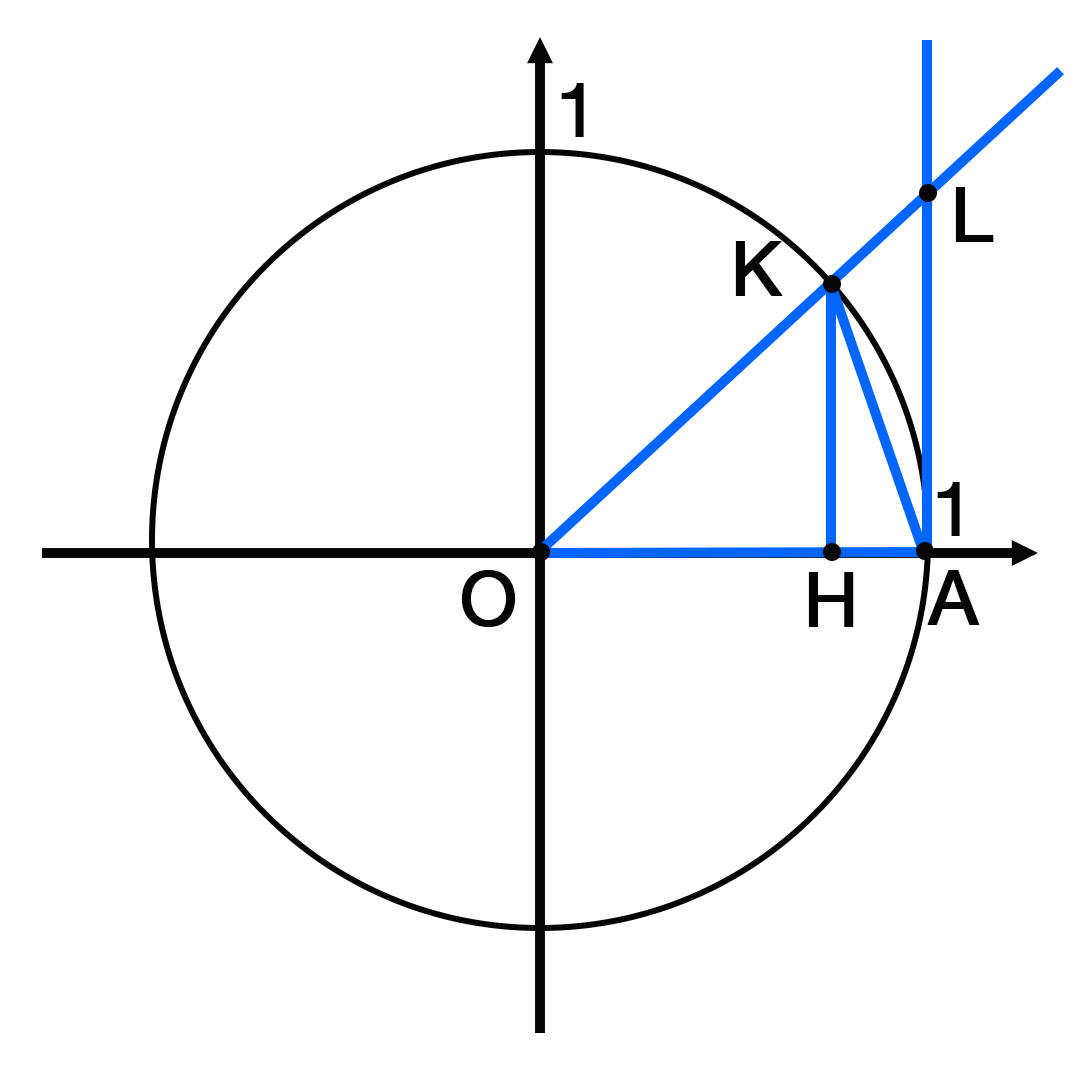
\includegraphics[width=0.6\textwidth]{limit_1.png}
\end{center}

Очевидно, что \(S_{\triangle OKA} < S_{sect KOA} < S_{\triangle OAL}\), где \(S_{sect KOA}\) — площадь сектора  \(KOA\). Поскольку \(|KH| = \sin{x}, |LA| = \tg{x}\):
\begin{gather*}
    S_{\triangle OKA} = \frac{1}{2} \cdot |OA| \cdot |KH| = \frac{1}{2} \cdot 1 \cdot \sin{x} = \frac{\sin{x}}{2} \\
    S_{sect KOA} = \frac{1}{2} \cdot |OA|^2 \cdot x = \frac{x}{2}                                                 \\
    S_{\triangle OAL} = \frac{1}{2} \cdot |OA| \cdot |LA| = \frac{\tg{x}}{2}
\end{gather*}
Тогда, заменив площади в неравенстве, получим:
\begin{gather*}
    \dfrac{\sin{x}}{2} < \dfrac{x}{2} < \dfrac{\tg{x}}{2}
\end{gather*}

Так как при \(x \to +0: \sin{x} > 0, x > 0, \tg{x} > 0\), получим:
\begin{gather*}
    \dfrac{1}{\tg{x}} < \dfrac{1}{x} < \dfrac{1}{\sin{x}} \iff \cos{x} < \dfrac{\sin{x}}{x} < 1
\end{gather*}

Перейдем к пределу:
\begin{gather*}
    \lim_{x \to +0}{\cos{x}} \leq \lim_{x \to +0}{\dfrac{\sin{x}}{x}} \leq 1 \implies 1 \leq \lim_{x \to +0}{\dfrac{\sin{x}}{x}} \leq 1 \implies \lim_{x \to +0}{\dfrac{\sin{x}}{x}} = 1
\end{gather*}

Найдем левый односторонний предел. Пусть \(t = -x \implies t \to +0\):
\begin{gather*}
    \lim_{x \to -0}{\dfrac{\sin{x}}{x}} = \lim_{t \to +0}{\dfrac{\sin{(-t)}}{-t}} = \lim_{t \to +0}{\dfrac{-\sin{t}}{-t}} = \lim_{t \to +0}{\dfrac{\sin{t}}{t}} = 1
\end{gather*}

Правый и левый односторонний пределы существуют и равны \(1\), следовательно и сам предел равен 1.

\subsubsection*{Следствия}
\begin{enumerate}
    \item {\(\lim_{x \to 0}{\dfrac{\tg{x}}{x}} = 1\)}
    \item {\(\lim_{x \to 0}{\dfrac{\arcsin{x}}{x}} = 1\)}
    \item {\(\lim_{x \to 0}{\dfrac{\arctg{x}}{x}} = 1\)}
    \item {\(\lim_{x \to 0}{\dfrac{1 - \cos{x}}{\frac{x^2}{2}}} = 1\)}
\end{enumerate}

\section{Второй замечательный предел. Число \(e\)}\label{sec:limit_2}
\begin{gather*}
    \lim_{x \to \infty}{\Big(1 + \frac{1}{x}\Big)^x} = e \text{ или } \lim_{x \to 0}{(1 + x)^\frac{1}{x}} = e
\end{gather*}

\begin{proof}
    Сначала докажем теорему для натуральных значений \(x\):
    \begin{gather*}
        x_n = \Big(1 + \frac{1}{n}\Big)^n; n \in \mathbb{N}
    \end{gather*}

    По формуле бинома Ньютона:
    \begin{align*}
        (a + b)^n & = a^n + \frac{n}{1} \cdot a^{n - 1} + \frac{n(n - 1)}{1 \cdot 2} \cdot a^{n - 2} \cdot b^2 + ... + \\
                  & + \frac{n(n - 1)(n - 2)...(n - (n - 1))}{1 \cdot 2 \cdot 3 \cdot ... \cdot n} \cdot b^n
    \end{align*}

    Полагая \(a = 1, b = \dfrac{1}{n}\), получим:
    \begin{align*}
        \Big(1 + \frac{1}{n}\Big)^n & = 1 + \frac{n}{1} \cdot \frac{1}{n} + \frac{n(n - 1)}{1 \cdot 2} \cdot \frac{1}{n^2} +
        \frac{n(n - 1)(n - 2)}{1 \cdot 2 \cdot 3} \cdot \frac{1}{n^3} + ... +                                                                                                                             \\
                                    & +                            \frac{n(n - 1)(n - 2)...(n - (n - 1))}{1 \cdot 2 \cdot 3 \cdot ... \cdot n} \cdot \frac{1}{n^n}                                        \\
        \Big(1 + \frac{1}{n}\Big)^n & = 1 + 1 + \frac{1}{1 \cdot 2} \cdot \Big(1 - \frac{1}{n}\Big) + \frac{1}{1 \cdot 2 \cdot 3} \cdot \Big(1 - \frac{1}{n}\Big) \cdot \Big(1 - \frac{2}{n}\Big) + ... + \\
                                    & + \frac{1}{1 \cdot 2 \cdot 3 ... \cdot n} \cdot \Big(1 - \frac{1}{n}\Big) \cdot \Big(1 - \frac{2}{n}\Big) \cdot ... \cdot \Big(1 - \frac{n - 1}{n}\Big)
    \end{align*}

    С увеличением \(n\) число полож. слагаемых в правой части увеличивается. Кроме того, при увеличении \(n\) число  \(\frac{1}{n}\) убывает. Следовательно величины \(\Big(1 - \dfrac{1}{n}\Big), \Big(1 - \dfrac{2}{n}\Big), ...\) возрастают, а значит и последовательность является возрастающей.

    Заметим, что \(\Big(1 + \frac{1}{n}\Big)^n \geq 2, n \in \mathbb{N}\).

    Покажем, что последовательность ограничена, заменив каждую скобку в правой части на единицу:
    \begin{gather*}
        \Big(1 + \frac{1}{n}\Big)^n < 1 + 1 + \frac{1}{1 \cdot 2} + \frac{1}{1 \cdot 2 \cdot 3} + ... + \frac{1}{1 \cdot 2 \cdot 3 \cdot ... \cdot n}
    \end{gather*}
    Усилим полученное неравенство, заменив \(3, 4, 5, ...\), стоящие в знаменателях дробей числом  \(2\) :
    \begin{gather*}
        \Big(1 + \frac{1}{n}\Big)^n < 1 + \Big(1 + \frac{1}{2} + \frac{1}{2^2} + ... + \frac{1}{2^{n - 1}}\Big)
    \end{gather*}

    Заметим, что в скобках получилась геометрическая прогрессия, сумма которой равна \(2 \cdot \Big(1 - \dfrac{1}{2^n}\Big) < 2>\). А значит:
    \begin{gather*}
        2 \leq \Big(1 + \frac{1}{n}\Big)^n < 3
    \end{gather*}

    На основании теоремы Вейерштрасса наша последовательность монотонно возрастает и ограничена, как следствие, имеет предел, равный \(e\):
    \begin{gather*}
        \lim_{n \to \infty}{\Big(1 + \frac{1}{n}\Big)^n} = e
    \end{gather*}
\end{proof}

\subsubsection*{Следствия}
\begin{enumerate}
    \item {\(\displaystyle{\lim_{x \to 0}{(1 + x)^{\frac{1}{x}}} = e}\)}
    \item {\(\displaystyle{\lim_{x \to \infty}{\Big(1 + \dfrac{k}{x}\Big)^x} = e^k}\)}
    \item {\(\displaystyle{\lim_{x \to 0}{\dfrac{\ln{(1 + x)}}{x}} = 1}\)}
    \item {\(\displaystyle{\lim_{x \to 0}{\dfrac{e^x - 1}{x}} = 1}\)}
    \item {\(\displaystyle{\lim_{x \to 0}{\dfrac{a^x - 1}{x\ln{a}} = 1}}\) для \(a > 0, a \neq 1\)}
    \item {\(\displaystyle{\lim_{x \to 0}{\dfrac{(1 + x)^k - 1}{kx}} = 1}\)}
\end{enumerate}

\subsection*{Число \(e\)}
Число \(e\) может быть определено несколькими способами:
\begin{itemize}
    \item {Через предел: \(e = \lim_{x \to \infty}{\Big(1 + \dfrac{1}{x}\Big)^x}\) или \(e = \lim_{n \to \infty}{\dfrac{n}{\sqrt[n]{n!}}}\) (следует из формулы Муавра-Стирлинга)}

    \item {Как сумма ряда: \(e = \displaystyle{\sum_{n = 0}^{\infty}{\dfrac{1}{n!}}}\) или \(\dfrac{1}{e} = \displaystyle{\sum_{n = 2}^{\infty}{\dfrac{(-1)^n}{n!}}}\) }

    \item {Как единственное число \(a\), для которого выполняется: \(\displaystyle{\int_{1}^{a}{\dfrac{dx}{x}} = 1}\)}

    \item {Как единственное полож. число \(a\), для которого верно: \(\dfrac{d}{dx}a^x = a^x\)}
\end{itemize}

\subsubsection*{Свойства}
\begin{enumerate}
    \item {Производная экспоненты равна самой экспоненте}
    \item {Число \(e\) иррационально}
    \item {Число \(e\) трансцендентно (не может быть корнем многочлена с целочисленными коэффицентами)}
    \item {\(e^{ix} = \cos{x} + i \cdot \sin{x}\)}
    \item {\(e^{i\pi} + 1 = 0\)}
    \item {Число \(e\) разлагается в бесконечную дробь}
\end{enumerate}

\section{Теоремы Вейерштрасса}%
\label{sec:Теоремы Вейерштрасса}

\begin{theorem}[Вейерштрасса для непрерывных функций]
    \newpar
    Если функция \(f(x)\) непрерывна на всем \([a, b]\), то она ограничена на нем и притом \(\exists \min{(f(x))}, \max{(f(x))}\), т. е. \(\exists \; x_m, x_M \in [a, b]: f(x_m) \leq f(x) \leq f(x_M) \; \forall x \in [a, b]\).
\end{theorem}

\begin{theorem}[Вейерштрасса для полунепрерывных функций]
    \newpar
    Если функция \(f(x): [a, b] \to \mathbb{R}\) ограничена и полунепрерывна \textbf{сверху}, то:
    \[
        \begin{cases}
            M = \underset{x \in [a, b]}{\sup}f(x) < +\infty \\
            \exists x_M \in [a, b]: f(x_M) = M
        \end{cases}
    \]

    Если функция \(f(x): [a, b] \to \mathbb{R}\) ограничена и полунепрерывна \textbf{снизу}, то:
    \[
        \begin{cases}
            m = \underset{x \in [a, b]}{\inf}f(x) > -\infty \\
            \exists x_m \in [a, b]: f(x_m) = m
        \end{cases}
    \]
\end{theorem}

\begin{proof}
    % TODO добавить доказательство
\end{proof}

\section{Теорема Ролля}%
\label{sec:Теорема Ролля}
\begin{theorem}[Ролля]
    Если функция \(f(x)\) непрерывна на \([a, b]\), дифференцируема на \((a, b)\) и \(f(a) = f(b)\), то найдется такая точка \(c \in (a, b)\), что \(f'(c) = 0\).
\end{theorem}

\begin{proof}
    Если \(f(x)\) постоянна на всем \([a, b]\), то утверждение верно и очевидно, поскольку \(f'(x) = 0 \; \forall x \in (a, b)\).

    Если же нет, поскольку \(f(a) = f(b)\), то согласно \plink{sec:Теоремы Вейерштрасса}{теореме Вейерштрасса}, \(\exists \min{(f(x)), \max{(f(x))}}\), то есть имеет в этой точке локальный экстремум, и по лемме Ферма производная в этой точке равна 0.

    Поскольку \(f(x)\) непрерывна на \([a, b]\)
\end{proof}

\section{Теоремы Лагранжа и Коши}%
\label{sec:Теоремы Лагранжа и Коши}
\begin{theorem}[Лагранжа]
    Если функция \(f(x)\) непрерывна на \([a, b]\) и дифференцируема на \((a, b)\), то найдется такая точка \(c \in (a, b)\), что
    \[
        \frac{f(b) - f(a)}{b - a} = f'(c).
    \]
\end{theorem}

\begin{theorem}[Коши]
    Пусть функции \(f(x)\) и \(g(x)\) непрерывны на \([a, b]\) и дифференцируемы на \((a, b)\), причем \(g'(x) \neq 0 \;\; \forall x \in (a, b)\). Тогда найдется такая точка \(c \in (a, b)\), что
    \[
        \frac{f(b) - f(a)}{g(b) - g(a)} = \frac{f'(c)}{g'(c)}.
    \]
\end{theorem}

\begin{note}
    Теорема Лагранжа — частный случай теоремы Коши, где \(g(x) = x\). Поэтому достаточно доказать теорему Коши.
\end{note}

\begin{proof}[теоремы Коши]
    Заметим, что \(g(a) \neq g(b)\), так как иначе по теореме Ролля \(\exists \; t \in (a, b): g'(t) = 0\).

    Введем новую функцию \(h(x) = f(x) - Kg(x)\), где \(K = \dfrac{f(b) - f(a)}{g(b) - g(a)}\). Также заметим, что \(h(a) = h(b)\), а потому функция \(h(x)\) удовлетворяет условиям теоремы Ролля. Значит, найдется такая точка \(c \in (a, b)\), что \(h'(c) = 0 \iff f'(c) = Kg'(c)\). Отсюда получим:
    \begin{gather*}
        K = \frac{f'(c)}{g'(c)} \iff \frac{f(b) - f(a)}{g(b) - g(a)} = \frac{f'(c)}{g'(c)}
    \end{gather*}
\end{proof}

\section{Правило Лопиталя}%
\label{sec:Правило Лопиталя}

Правило Лопиталя действует одинаково как для неопределенности вида \(0/0\), так и для \(\infty/\infty\).
Однако их доказательства несколько различаются, поэтому они будут рассмотрены отдельно.

\begin{theorem}[«Правило Лопиталя» (\(0/0\) и  \(\infty/\infty\))]
    \newpar \vspace{0.1cm}
    Если функции \(f(x)\) и \(g(x)\) определены на \([a, b]\), дифференцируемы на \((a, b)\) и для них выполняются следующие условия:
    \begin{enumerate}[leftmargin=3em]
        \item {\(\displaystyle\lim_{x \to a}{f(x)} = \lim_{x \to a}{g(x)} = 0 \text{ или } \infty\)}
        \item {\(g'(x) \neq 0 \; \forall x \in (a, b)\)}
        \item {\(\displaystyle \exists \lim_{x \to a}{\dfrac{f'(x)}{g'(x)}}\)}
    \end{enumerate}

    Тогда существует \(\displaystyle\lim_{x \to a}{\dfrac{f(x)}{g(x)}} = \lim_{x \to a}{\dfrac{f'(x)}{g'(x)}}\)
\end{theorem}

\begin{proof}[первого правила Лопиталя (\(0/0\))]
    Доопределим или переопределим функции \(f(x)\) и \(g(x)\) в точке \(a\):
    \[
        f(a) = g(a) = 0
    \]

    На пределы и производные это никак не повлияет, поскольку они не зависят от того, чему равны функции в точке \(a\). Тогда по \plink{sec:Теоремы Лагранжа и Коши}{теореме Коши}:
    \[
        \frac{f(x)}{g(x)} =
        \frac{f(x) - f(a)}{g(x) - g(a)} =
        \frac{f'(c)}{g'(c)}
    \]

    где \(c \in (a, x)\).

    Поскольку существует \(\displaystyle \lim_{x \to a}{\dfrac{f'(x)}{g'(x)}}\), который равен
    \[
        \lim_{x \to a}{\frac{f(x)}{g(x)}} =
        \lim_{x \to a}{\frac{f'(c)}{g'(c)}}
    \]

    Если \(x \to a\), то и \(c \to a\), т. к. \(a < c < x\), следовательно:
    \[
        \lim_{x \to a}{\frac{f(x)}{g(x)}} =
        \lim_{x \to a}{\frac{f'(c)}{g'(c)}} =
        \lim_{x \to a}{\frac{f'(x)}{g'(x)}}.
    \]
\end{proof}

\begin{proof}[второго правила Лапиталя (\(\infty/\infty\))]
    Функции \(\dfrac{1}{f(x)}\) и \(\dfrac{1}{g(x)}\) являются бесконечно малыми при \(x \to a\). Тогда по первому правилу Лопиталя:
    \begin{gather*}
        \lim_{x \to a}{\frac{f(x)}{g(x)}} =
        \lim_{x \to a}{\frac{\dfrac{1}{g(x)}}{\dfrac{1}{f(x)}}} =
        \lim_{x \to a}{\frac{\Big(\dfrac{1}{g(x)}\Big)'}{\Big(\dfrac{1}{f(x)}\Big)'}} =
        \lim_{x \to a}{\frac{\dfrac{g'(x)}{g^2(x)}}{\dfrac{f'(x)}{f^2(x)}}} =
        \lim_{x \to a}{\frac{g'(x)f^2(x)}{f'(x)g^2(x)}} =
        \lim_{x \to a}{\frac{g'(x)}{f'(x)}} \cdot \Big(\lim_{x \to a}{\frac{f(x)}{g(x)}}\Big)^2
    \end{gather*}
    Следовательно:
    \begin{gather*}
        \lim_{x \to a}{\frac{f(x)}{g(x)}} =
        \lim_{x \to a}{\frac{g'(x)}{f'(x)}} \cdot \Big(\lim_{x \to a}{\frac{f(x)}{g(x)}}\Big)^2 \\
        \lim_{x \to a}{\frac{f(x)}{g(x)}} =
        \lim_{x \to a}{\frac{f'(x)}{g'(x)}}
    \end{gather*}
\end{proof}

\section{Теорема Ферма}%
\label{sec:Теорема Ферма}

\begin{theorem}[Ферма]
    Если функция \(f(x)\) определена и дифференцируема на \((a, b)\) и \(f(c) = \max(f(x))\) или \(f(c) = \min(f(x))\), где \(c \in (a, b)\), тогда \(f'(c) = 0\).
\end{theorem}

\begin{proof}
    Рассмотрим случай, когда \(f(c) = \max(f(x))\). Случай, когда \(c\) — точка минимума, доказывается аналогично. Производная \(f'(c)\) равна:
    \[
        f'(c) = \lim_{\Delta x \to 0}{\frac{f(c + \Delta x) - f(c)}{\Delta x}}
    \]
    \begin{gather*}
        \begin{cases}
            \Delta x > 0 \implies \dfrac{f(c + \Delta x) - f(c)}{\Delta x} \leq 0 \implies f'(c) \leq 0 \vspace{0.3cm} \\
            \Delta x < 0 \implies \dfrac{f(c + \Delta x) - f(c)}{\Delta x} \geq 0 \implies f'(c) \geq 0
        \end{cases}
        \implies f'(c) = 0
    \end{gather*}
\end{proof}

\end{document}
